\documentclass{article}%
\usepackage[T1]{fontenc}%
\usepackage[utf8]{inputenc}%
\usepackage{lmodern}%
\usepackage{textcomp}%
\usepackage{lastpage}%
%
\usepackage{amsmath}%
\usepackage{amssymb}%
\usepackage{amsfonts}%
\usepackage{graphicx}%
\usepackage{hyperref}%
\usepackage{tikz}%
\usepackage{pgfplots}%
\usetikzlibrary{math}%
\title{ITA 2027 - Química\thanks{This exam was solved and automatically generated with gpt-resolve: \url{https://github.com/lgabs/gpt-resolve}}}%
\author{claude{-}haiku{-}5{-}5 (solver) + claude{-}haiku{-}5{-}5 (judge)}%
\date{November 09, 2026}%
%
\begin{document}%
\normalsize%
\maketitle%
\section*{Questão 1}

\section*{Solução}

\textbf{Hipóteses e convenções.}
\begin{itemize}
\item Gases ideais. A composição do ar, dada em volume, equivale à fração molar: 20\% de O$_2$ e 80\% de N$_2$.
\item Pentano admitido como vapor a $T_i=300{,}84\,\text{K}$ ($\approx27{,}7\,^{\circ}\text{C}$). Esta é uma hipótese de modelagem, não um dado do enunciado: a 1 bar o pentano ferve por volta de 36 $^{\circ}$C, e, se entrasse líquido, seria preciso somar a entalpia de vaporização, que o enunciado não fornece. Por isso a vaporização não entra no balanço.
\item Todos os produtos são gasosos, inclusive H$_2$O, como indica a listagem da mistura gasosa no enunciado.
\item $\Delta H_c=-3440\,\text{kJ}\cdot\text{mol}^{-1}$ é tomada em $T_i$ e considerada constante no intervalo. Reação isobárica: $q_p=\Delta H$. Todo o calor liberado fica nos gases, de modo que o processo global não troca calor com o exterior (adiabático).
\item $C_p=40\,\text{J}\cdot\text{K}^{-1}\cdot\text{mol}^{-1}$ por mol de mistura gasosa, válido para misturas de composição variável e constante no intervalo de temperatura. A unidade impressa $\text{J}^{-1}\cdot\text{K}^{-1}\cdot\text{mol}^{-1}$ é erro de impressão: só $\text{J}\cdot\text{K}^{-1}\cdot\text{mol}^{-1}$ torna $Q=n\,C_p\,\Delta T$ uma energia.
\item Sinal: $\Delta H<0$ para a reação; o calor absorvido pelos gases é $Q=-n\,\Delta H_c>0$.
\end{itemize}

\textbf{a) Equação balanceada.} Com 1 mol de C$_5$H$_{12}$ e coeficientes $a$ (O$_2$), $b$ (CO$_2$) e $c$ (H$_2$O): balanço de C, $b=5$; de H, $2c=12$, logo $c=6$; de O, $2a=2b+c=16$, logo $a=8$.
\[
\mathrm{C_5H_{12}(g)}+8\,\mathrm{O_2(g)}\rightarrow 5\,\mathrm{CO_2(g)}+6\,\mathrm{H_2O(g)}
\]
Conferência: 5 C, 12 H e 16 O em cada lado.

\textbf{b) Quantidades de O$_2$ e N$_2$.} A admissão de ar é fixa e o volume do combustível injetado é desprezível frente aos 200 L, logo a quantidade de O$_2$ e de N$_2$ não depende da quantidade de combustível. Pela equação de Clapeyron, em SI coerente ($\text{Pa}\cdot\text{m}^3=\text{J}$), com $P=1{,}00\times10^{5}\,\text{Pa}$ (1 bar), $V=0{,}200\,\text{m}^3$ e $R=8{,}31\,\text{J}\cdot\text{K}^{-1}\cdot\text{mol}^{-1}$:
\[
n_{\text{ar}}=\frac{PV}{RT_i}=\frac{1{,}00\times10^{5}\cdot0{,}200}{8{,}31\cdot300{,}84}\,\text{mol}\approx\frac{2{,}00\times10^{4}}{2{,}50\times10^{3}}\,\text{mol}=8{,}00\,\text{mol}
\]
\[
n_{\mathrm{O_2}}=0{,}20\cdot8{,}00=1{,}6\,\text{mol}\qquad n_{\mathrm{N_2}}=0{,}80\cdot8{,}00=6{,}4\,\text{mol}
\]
Conferência com outras unidades: $1\,\text{bar}\approx0{,}987\,\text{atm}$ e $R=8{,}21\times10^{-2}\,\text{atm}\cdot\text{L}\cdot\text{K}^{-1}\cdot\text{mol}^{-1}$ dão $n_{\text{ar}}\approx7{,}99$ mol, com os mesmos valores. Tratar 1 bar como 1 atm daria $n_{\text{ar}}\approx8{,}10$ mol e $n_{\mathrm{N_2}}\approx6{,}5$ mol, erro que a conversão evita.

\textbf{c) Condição estequiométrica.} O O$_2$ é o reagente limitante: são necessários 8 mol de O$_2$ por mol de pentano, e há 1,6 mol. Logo $n_{\mathrm{C_5H_{12}}}=1{,}6/8=0{,}20$ mol, com todo o O$_2$ consumido e nenhum reagente em excesso.

Calor liberado a $T_i$:
\[
Q=-n\,\Delta H_c=-0{,}20\cdot(-3440)\,\text{kJ}=+688\,\text{kJ}=6{,}88\times10^{5}\,\text{J}
\]
Gases após a combustão: $n_{\mathrm{CO_2}}=5\cdot0{,}20=1{,}0$ mol; $n_{\mathrm{H_2O}}=6\cdot0{,}20=1{,}2$ mol; $n_{\mathrm{N_2}}=6{,}4$ mol; $n_{\mathrm{O_2}}=0$. Total $n_f=8{,}6$ mol.

Balanço: como o processo é isobárico e adiabático, $q_p=0=\Delta H_{\text{global}}$. Pela lei de Hess (entalpia é função de estado), o caminho reagentes a $T_i$ $\rightarrow$ produtos a $T_i$ $\rightarrow$ produtos a $T_f$ fornece
\[
0=\Delta H_{\text{rx}}(T_i)+n_f\,C_p\,(T_f-T_i)
\]
\[
\Rightarrow\ \Delta T=\frac{6{,}88\times10^{5}\,\text{J}}{8{,}6\cdot40\,\text{J}\cdot\text{K}^{-1}}=\frac{6{,}88\times10^{5}}{344}\,\text{K}=2000\,\text{K}
\]
\[
T_f=T_i+\Delta T=300{,}84+2000=2300{,}84\,\text{K}
\]
Sanidade: $\Delta T\approx2\times10^{3}$ K e $T_f-273{,}15\approx2028\,^{\circ}\text{C}$, ordem de grandeza plausível para chamas de hidrocarbonetos no ar. O resultado é uma estimativa do modelo: a dissociação dos produtos, ignorada, reduziria $T_f$, e o $C_p$ real varia com a temperatura.

\textbf{d) Redução de combustível para $T_f=1600{,}84$ K.} Seja $x$ a quantidade de C$_5$H$_{12}$, em mol. Como o O$_2$ é fixo em 1,6 mol, a combustão completa exige $8x\le1{,}6$, isto é, $x\le0{,}20$ mol. A elevação de temperatura pedida é $\Delta T=1600{,}84-300{,}84=1300$ K.

\emph{Ramo pobre} ($0<x\le0{,}20$): todo o pentano queima e sobra O$_2$. Os gases são $5x$ mol de CO$_2$, $6x$ de H$_2$O, $6{,}4$ de N$_2$ e $(1{,}6-8x)$ de O$_2$. Logo
\[
n_g=5x+6x+6{,}4+(1{,}6-8x)=8+3x,\qquad Q=3440\,x\ \text{kJ}=3{,}44\times10^{6}\,x\ \text{J}
\]
A composição varia com $x$, e o $C_p$ de 40 J$\cdot$K$^{-1}\cdot$mol$^{-1}$ vale por mol de mistura para qualquer composição; portanto o número de mols $n_g$ deve variar com $x$. Fixar $n_g=8{,}6$ mol seria aproximação que ignora essa variação (ver observação abaixo).

Balanço $Q=n_g\,C_p\,\Delta T$:
\[
3{,}44\times10^{6}\,x=(8+3x)\cdot40\cdot1300=416000+156000\,x
\]
\[
\Rightarrow\ 3284000\,x=416000\ \Rightarrow\ x=\frac{104}{821}\approx0{,}1267\ \text{mol}
\]
Unicidade: $\Delta T(x)=\dfrac{86000\,x}{8+3x}$ tem derivada $\dfrac{8\cdot86000}{(8+3x)^2}>0$, é estritamente crescente em $(0;0{,}20]$ e varia de 0 a 2000 K. Logo a solução é única nesse ramo.

Em relação à estequiometria, $x/0{,}20\approx0{,}633$, ou seja, 63\% da quantidade estequiométrica. A variação é $63{,}3\%-100\%=-36{,}7\%$, que arredonda para $-37\%$.

Verificação: o O$_2$ remanescente é $1{,}6-8\cdot0{,}1267\approx0{,}59$ mol $>0$, coerente com o ramo pobre. Além disso, $n_g=8+3\cdot0{,}1267\approx8{,}38$ mol, $Q=3440\cdot0{,}1267\approx4{,}36\times10^{5}$ J e $\Delta T=\dfrac{4{,}36\times10^{5}}{40\cdot8{,}38}\approx1300$ K.

Observação: se $n_g$ fosse fixado em 8,6 mol, obter-se-ia $x=0{,}13$ mol (65\%, redução de 35\%). Esse valor é aproximado, pois ignora a variação da composição que o enunciado explicita; não é o resultado adotado.

\emph{Ramo rico} ($x>0{,}20$, excluído): o O$_2$ limita a combustão a 0,20 mol de pentano ($Q=688$ kJ), e os $(x-0{,}20)$ mol restantes não queimam. Como estimativa de modelo simplificado, tratam-se como inertes aquecidos com $C_p$; a combustão parcial (CO, H$_2$) não é considerada. Então $n_g=8{,}6+(x-0{,}20)=8{,}4+x$ e
\[
6{,}88\times10^{5}=40\cdot1300\,(8{,}4+x)\ \Rightarrow\ 8{,}4+x\approx13{,}23\ \Rightarrow\ x\approx4{,}83\ \text{mol}
\]
Isso equivale a cerca de 24 vezes a quantidade estequiométrica (aumento de cerca de 2315\%). Esse ramo contraria a hipótese de combustão completa e exige muito mais combustível, o oposto da economia pedida. Assim, a combustão completa e a economia de combustível selecionam o ramo pobre.

\textbf{Resultado do item d:} a quantidade de pentano deve ser reduzida em 37\% em relação à estequiométrica, ficando com 63\% dela ($x\approx0{,}127$ mol).

ANSWER: (a) $\mathrm{C_5H_{12}(g)}+8\,\mathrm{O_2(g)}\rightarrow 5\,\mathrm{CO_2(g)}+6\,\mathrm{H_2O(g)}$; (b) $n_{\mathrm{O_2}}=1{,}6$ mol e $n_{\mathrm{N_2}}=6{,}4$ mol; (c) $T_f=2300{,}84$ K ($\Delta T=2000$ K); (d) redução de $37\%$ (pentano a $63\%$ da quantidade estequiométrica, $x\approx0{,}127$ mol).%
\newpage%
\section*{Questão 2}

\section*{Solução}

\textbf{Hipóteses e modelo.}
\begin{enumerate}
\item Supõe-se que a substância seja molecular e não ionizável, logo $i=1$ (o enunciado não informa dissociação).
\item A membrana é ideal: só o solvente a atravessa. O soluto, inclusive o sólido que eventualmente precipite, permanece no compartimento da solução.
\item O processo é isotérmico ($T=305\,\mathrm{K}$), quase-estático e reversível. A cada instante, a pressão aplicada ao êmbolo da solução é $P_{\mathrm{atm}}+\pi$, com $\pi$ a pressão osmótica naquele instante; o solvente puro está sob $P_{\mathrm{atm}}$. Assim, a diferença de pressão através da membrana é $\pi$, e $P_{\mathrm{atm}}$ se cancela.
\item A solução é diluída e ideal, valendo $\pi=cRT$, com $c$ em $\mathrm{mol\,L^{-1}}$ e $R=8{,}21\times 10^{-2}\,\mathrm{atm\,L\,K^{-1}\,mol^{-1}}$. As concentrações entram como $c/c^{\circ}$, com $c^{\circ}=1\,\mathrm{mol\,L^{-1}}$, numericamente iguais a $c$.
\item Na saturação, a fração molar do soluto é $\approx 0{,}05/55{,}5\approx 9\times 10^{-4}$, o que justifica a aproximação diluída.
\item A solubilidade de $4\,\mathrm{g\,L^{-1}}$ é a concentração de saturação a $305\,\mathrm{K}$. Acima dela, o excesso precipita como sólido puro, de atividade unitária.
\item Geometria: $A=1\,\mathrm{dm^2}$ nos dois compartimentos. Descer o êmbolo da solução de $d$ dm reduz o volume de solução em $A\,d=d\,\mathrm{L}$; o mesmo volume de solvente atravessa a membrana e eleva o êmbolo do solvente de $d$ dm.
\item Membrana: pela figura (esquemática, leitura aproximada da escala), ela é a faixa escura no canal inferior de ligação, entre cerca de $7{,}5$ e $9$ dm. Para $d\le 7{,}5$ dm, toda a membrana está em contato com a solução; para $7{,}5<d<9$ dm, essa área diminui até zero em $d=9$ dm. A área altera apenas a velocidade de passagem do solvente, não o equilíbrio que define $\pi$; o limite de 9 dm é coerente com o fim do contato.
\item Desprezam-se a pressão hidrostática (o enunciado não fornece $\rho$ nem $g$) e os volumes do soluto e do sólido (da ordem de 1\% do volume da solução). A hidrostática alteraria a pressão que o êmbolo precisa exercer, não a pressão osmótica $cRT$.
\end{enumerate}

\textbf{Passo 1: volumes, concentrações e saturação.}
\begin{align*}
V_0 &= A\,h_0=(1\,\mathrm{dm^2})(10\,\mathrm{dm})=10\,\mathrm{dm^3}=10\,\mathrm{L}\\
c_0 &= \frac{n}{V_0}=\frac{0{,}2\,\mathrm{mol}}{10\,\mathrm{L}}=0{,}020\,\mathrm{mol\,L^{-1}}\qquad(\text{ou } 1{,}6\,\mathrm{g\,L^{-1}})\\
c_{\mathrm{sat}} &= \frac{4\,\mathrm{g\,L^{-1}}}{80\,\mathrm{g\,mol^{-1}}}=0{,}050\,\mathrm{mol\,L^{-1}}
\end{align*}
Comparando em g/L, $1{,}6<4$; em mol/L, $0{,}020<0{,}050$. A solução inicial é insaturada e não há sólido.

\textbf{Passo 2: de onde vem $\pi=cRT$.} No equilíbrio do solvente através da membrana, seu potencial químico na solução, sob $P_{\mathrm{atm}}+\pi$, iguala o do solvente puro sob $P_{\mathrm{atm}}$. Com volume molar $\bar V_w$ constante (líquido praticamente incompressível),
\[
\mu_w^{*}(P_{\mathrm{atm}})+\bar V_w\,\pi+RT\ln a_w=\mu_w^{*}(P_{\mathrm{atm}})
\quad\Rightarrow\quad
\pi=-\frac{RT}{\bar V_w}\,\ln a_w
\]
Para solução diluída, $a_w\approx x_w=1-x_s$ e $-\ln x_w\approx x_s$. Como $x_s\approx n_s/n_w$ e $n_w\bar V_w\approx V$, resulta $x_s/\bar V_w\approx n_s/V=c$, logo $\pi\approx cRT$. Assim, $\pi$ depende apenas de $a_w$, isto é, da fração molar do soluto.

\textbf{Passo 3: solução insaturada, $0\le d\le 6$ dm.} Enquanto $c<c_{\mathrm{sat}}$, todo o soluto permanece dissolvido: $n=0{,}2$ mol é constante e $V(d)=(10-d)\,\mathrm{L}$ (pois $1\,\mathrm{dm^3}=1\,\mathrm{L}$). Então
\[
\pi(d)=\frac{nRT}{V(d)}=\frac{0{,}2\times 8{,}21\times 10^{-2}\times 305}{10-d}\approx\frac{5{,}01}{10-d}\,\mathrm{atm}\qquad(d\ \mathrm{em\ dm})
\]
Unidades: $\mathrm{mol}\cdot\mathrm{atm\,L\,K^{-1}\,mol^{-1}}\cdot\mathrm{K}/\mathrm{L}=\mathrm{atm}$. Em $d=0$, $\pi_0=c_0RT=0{,}020\times 8{,}21\times 10^{-2}\times 305\approx 0{,}50$ atm; a curva não parte da origem.

\textbf{Passo 4: ponto de saturação.} A concentração atinge $c_{\mathrm{sat}}$ quando
\[
V^{*}=\frac{n}{c_{\mathrm{sat}}}=\frac{0{,}2}{0{,}050}=4{,}0\,\mathrm{L}\quad\Rightarrow\quad d^{*}=10-4{,}0=6{,}0\,\mathrm{dm}
\]
Nesse ponto, $\pi^{*}=c_{\mathrm{sat}}RT\approx 1{,}25$ atm, coincidindo com $5{,}01/4{,}0\approx 1{,}25$ atm. A derivada $d\pi/dd=nRT/(10-d)^2\approx 0{,}31$ atm/dm para $d\to 6^{-}$ e vale zero depois: a curva forma uma quina em $d^{*}$.

\textbf{Passo 5: solução saturada, $6\le d\le 9$ dm.} Com sólido presente, o potencial químico do soluto na solução iguala o do sólido puro (atividade unitária). Logo a atividade do soluto, e na solução diluída a concentração, fica fixa em $c_{\mathrm{sat}}$. Então $x_s$ e, pela relação do Passo 2, $a_w$ e $\pi$ também ficam fixos:
\[
\pi(d)=c_{\mathrm{sat}}RT\approx 1{,}25\,\mathrm{atm}\qquad(6\le d\le 9\ \mathrm{dm})
\]
A solução restante ocupa $(10-d)$ L e dissolve $0{,}050\,(10-d)$ mol. O excesso precipita:
\[
n_{\mathrm{sól}}=0{,}2-0{,}050\,(10-d)=0{,}050\,d-0{,}30\ \mathrm{mol}\quad\Rightarrow\quad m_{\mathrm{sól}}=80\,n_{\mathrm{sól}}=(4d-24)\ \mathrm{g}
\]
Em $d=9$ dm, há 0,15 mol (12 g) de sólido. Sem precipitação, $\pi$ cresceria sem limite à medida que $V\to 0$ (em $d\to 10$ dm); é a precipitação que fixa $\pi$.

\textbf{Passo 6: função, tabela e gráfico.}
\[
\pi(d)=
\begin{cases}
\dfrac{5{,}01}{10-d}\,\mathrm{atm}, & 0\le d\le 6\ \mathrm{dm}\\[2ex]
1{,}25\,\mathrm{atm}, & 6\le d\le 9\ \mathrm{dm}
\end{cases}
\]

\begin{center}
\begin{tabular}{|c|c|c|c|c|}
\hline
$d$ (dm) & $V$ (L) & $[X]$ (mol\,L$^{-1}$) & $\pi$ (atm) & massa precipitada (g) \\
\hline
0 & 10 & $0{,}020$ & $0{,}50$ & 0 \\
1 & 9 & $0{,}022$ & $0{,}56$ & 0 \\
2 & 8 & $0{,}025$ & $0{,}63$ & 0 \\
3 & 7 & $0{,}029$ & $0{,}72$ & 0 \\
4 & 6 & $0{,}033$ & $0{,}83$ & 0 \\
5 & 5 & $0{,}040$ & $1{,}00$ & 0 \\
6 & 4 & $0{,}050$ & $1{,}25$ & 0 \\
7 & 3 & $0{,}050$ & $1{,}25$ & 4 \\
8 & 2 & $0{,}050$ & $1{,}25$ & 8 \\
9 & 1 & $0{,}050$ & $1{,}25$ & 12 \\
\hline
\end{tabular}
\end{center}

\pgfplotsset{compat=1.18, /pgf/number format/use comma}
\begin{center}
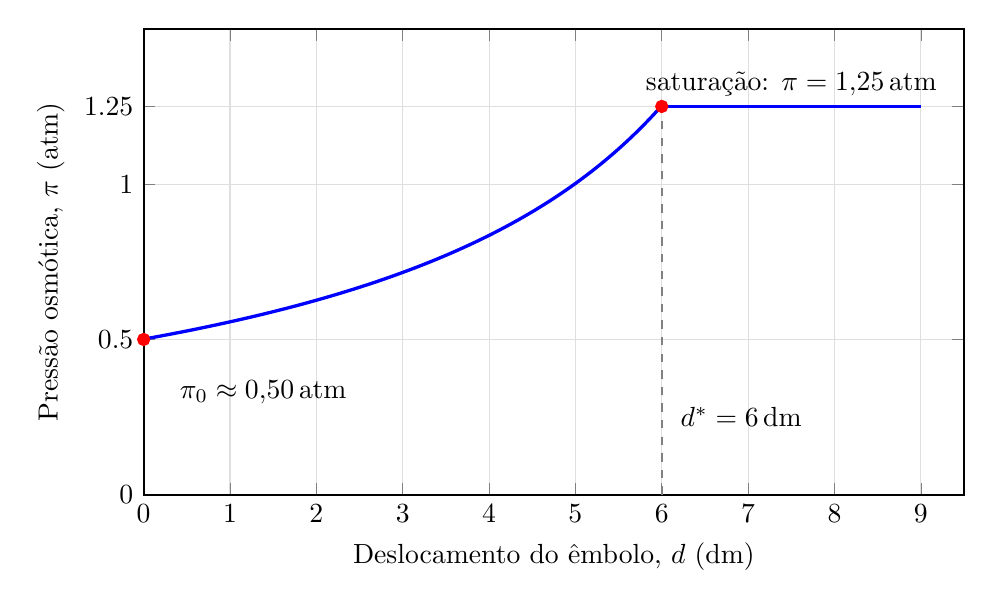
\begin{tikzpicture}
\begin{axis}[
    width=12cm, height=7.5cm,
    xmin=0, xmax=9.5, ymin=0, ymax=1.5,
    xtick={0,1,2,3,4,5,6,7,8,9},
    ytick={0,0.5,1,1.25},
    xlabel={Deslocamento do êmbolo, $d$ (dm)},
    ylabel={Pressão osmótica, $\pi$ (atm)},
    grid=major, grid style={gray!25},
    thick,
]
\addplot[blue, very thick, domain=0:6, samples=120] {5.01/(10-x)};
\addplot[blue, very thick, domain=6:9] {1.25};
\addplot[only marks, mark=*, mark size=2pt, red] coordinates {(0,0.50) (6,1.25)};
\draw[dashed, gray] (axis cs:6,0) -- (axis cs:6,1.25);
\node[anchor=west] at (axis cs:0.3,0.33) {$\pi_0\approx 0{,}50$\,atm};
\node[anchor=west] at (axis cs:6.1,0.25) {$d^{*}=6$\,dm};
\node[anchor=south] at (axis cs:7.5,1.25) {saturação: $\pi=1{,}25$\,atm};
\end{axis}
\end{tikzpicture}
\end{center}

O gráfico tem dois trechos: de $d=0$ a $d=6$ dm, $\pi$ cresce segundo a hipérbole de $0{,}50$ a $1{,}25$ atm; de $d=6$ a $d=9$ dm, $\pi$ é constante.

\textbf{Verificações.}
\begin{itemize}
\item Continuidade em $d=6$ dm: $5{,}01/4{,}0\approx 1{,}25$ atm $=c_{\mathrm{sat}}RT$.
\item Início: $\pi(0)=0{,}50$ atm $\neq 0$.
\item Ordem de grandeza: a 305 K, $RT\approx 25\,\mathrm{atm\,L\,mol^{-1}}$, logo $0{,}05\times 25\approx 1{,}25$ atm.
\item Sentido: $\pi$ cresce porque o solvente sai da solução e a concentra. Na osmose reversa, a pressão aplicada $P_{\mathrm{atm}}+\pi$ é o limiar reversível do fluxo.
\end{itemize}

ANSWER: $\pi(d)=\dfrac{5{,}01}{10-d}\,\mathrm{atm}$ para $0\le d\le 6\,\mathrm{dm}$ (de $0{,}50$ a $1{,}25\,\mathrm{atm}$) e $\pi=1{,}25\,\mathrm{atm}$ constante para $6\le d\le 9\,\mathrm{dm}$; a solução satura em $d=6\,\mathrm{dm}$ e o excesso precipita, chegando a $12\,\mathrm{g}$ em $d=9\,\mathrm{dm}$.%
\newpage%
\section*{Questão 3}

\section*{Solução}

\textbf{Reagente.} O álcool é o 2-metilbutan-2-ol, $(\mathrm{CH_3})_2\mathrm{C(OH){-}CH_2CH_3}$ ($\mathrm{C_5H_{12}O}$), com OH em carbono terciário. Na cadeia, C1 é uma das metilas de C2 (a outra é substituinte), C3 é o $\mathrm{CH_2}$ e C4 o $\mathrm{CH_3}$ terminal.

\textbf{a) X: desidratação por E1.} O enunciado não dá a concentração do $\mathrm{H_2SO_4}$; adota-se a condição usual de desidratação (ácido forte, aquecimento), em que o ácido é catalisador. Etapas:
\begin{enumerate}
\item protonação rápida da hidroxila (equilíbrio ácido-base):
\[ \mathrm{R{-}OH + H^{+} \rightleftharpoons R{-}OH_2^{+}} \]
\item saída de água, lenta e determinante da velocidade, gerando o carbocátion terciário $\mathrm{(CH_3)_2C^{+}{-}CH_2CH_3}$:
\[ \mathrm{R{-}OH_2^{+} \rightarrow R^{+} + H_2O} \]
\item perda de $\mathrm{H^{+}}$ de carbono vizinho, por $\mathrm{H_2O}$ ou $\mathrm{HSO_4^{-}}$, regenerando o catalisador.
\end{enumerate}
\textit{Rearranjo.} Não ocorre: o carbocátion já é terciário, e os deslocamentos 1,2 de H ou de $\mathrm{CH_3}$ levariam a carbocátions secundário ou primário.

\textit{Eliminação.} Perda de H de C3 dá o 2-metilbut-2-eno (trissubstituído); perda de H de C1 dá o 2-metilbut-1-eno (dissubstituído). Pela regra de Saytzeff, o alceno mais substituído, mais estável por hiperconjugação, é o majoritário. Como o enunciado trata X como um único símbolo, adota-se esse majoritário. A escolha é convencional, e os itens c) e d) dependem dela (ver a sensibilidade).
\[ X = (\mathrm{CH_3})_2\mathrm{C{=}CH{-}CH_3} \]
2-metilbut-2-eno, $\mathrm{C_5H_{10}}$, sem isomeria E/Z (C2 tem duas metilas iguais).

\textit{Por que não o éter.} (i) A via $\mathrm{S_N2}$ é impedida em carbono terciário. (ii) Na via $\mathrm{S_N1}$, o álcool, nucleófilo fraco e volumoso, ataca mal o carbocátion, e a quente a eliminação é favorecida pela entropia: 1 molécula de álcool gera 2 (alceno e água), com $\Delta S > 0$. Já $2\,\mathrm{ROH \rightarrow ROR + H_2O}$ mantém o número de moléculas ($\Delta S \approx 0$).

Balanço: $\mathrm{C_5H_{12}O \rightarrow C_5H_{10} + H_2O}$ (C: 5 = 5; H: 12 = 10 + 2; O: 1 = 1).

\textbf{b) Z: adição iônica de HBr (Markovnikov).} O $\mathrm{H^{+}}$ liga-se ao C3 (menos substituído), gerando o carbocátion terciário em C2; o $\mathrm{Br^{-}}$ ataca esse carbocátion, sem rearranjo, como em a).
\[ (\mathrm{CH_3})_2\mathrm{C{=}CH{-}CH_3} + \mathrm{HBr} \rightarrow (\mathrm{CH_3})_2\mathrm{CBr{-}CH_2CH_3} \]
Z = 2-bromo-2-metilbutano, $\mathrm{C_5H_{11}Br}$, aquiral (C2 tem duas metilas iguais).

\textbf{c) G: adição radicalar de HBr (anti-Markovnikov, efeito Kharasch).} Com peróxido:
\begin{itemize}
\item iniciação (homólise fraca da ligação O-O e abstração de H do HBr pelo radical hidroxila):
\[ \mathrm{H_2O_2 \rightarrow 2\,HO^{\bullet}} \qquad \mathrm{HO^{\bullet} + HBr \rightarrow H_2O + Br^{\bullet}} \]
\item propagação: $\mathrm{Br^{\bullet}}$ adiciona-se ao C3, formando o radical terciário em C2 (mais estável); esse radical retira H de HBr, regenerando $\mathrm{Br^{\bullet}}$. A etapa é exotérmica, pois a ligação C-H formada é mais forte que a H-Br rompida.
\end{itemize}
\[ (\mathrm{CH_3})_2\mathrm{C{=}CH{-}CH_3} + \mathrm{HBr} \xrightarrow{\text{peróxido}} (\mathrm{CH_3})_2\mathrm{CH{-}CHBr{-}CH_3} \]
G = 2-bromo-3-metilbutano, $\mathrm{C_5H_{11}Br}$. Os localizadores são {2,3} numerando a cadeia por qualquer extremidade; o empate vai para o substituinte que vem primeiro em ordem alfabética (bromo), que recebe o localizador 2.

Estereoquímica: o CHBr (C2 de G) tem quatro grupos diferentes e é o único estereocentro. Ele é formado na adição do $\mathrm{Br^{\bullet}}$ ao alceno plano e aquiral, que ataca por uma ou outra face com igual probabilidade (as faces são enantiotópicas e não há indução quiral). Obtêm-se R e S em partes iguais: mistura racêmica. O radical terciário, também plano, não define essa configuração, pois o carbono radicalar (C3 de G) não é estereogênico, com duas metilas iguais. O efeito é específico do HBr: com HCl, a abstração de H é endotérmica; com HI, o peróxido é reduzido.

\textbf{d) J: hidroxilação sin (teste de Baeyer).} Com $\mathrm{KMnO_4}$ diluído, a frio e em meio básico, o $\mathrm{MnO_4^{-}}$ adiciona-se pela mesma face da dupla, formando um éster cíclico de manganato(V), em que o Mn é Mn(V). A hidrólise libera o diol cis, e o manganês é reduzido a $\mathrm{MnO_2}$ (Mn(IV)); o balanço é de 3 elétrons por $\mathrm{MnO_4^{-}}$ (Mn(VII) $\rightarrow$ Mn(IV)). As condições brandas evitam a clivagem oxidativa, que ocorre com $\mathrm{KMnO_4}$ concentrado e quente.
\[ (\mathrm{CH_3})_2\mathrm{C{=}CH{-}CH_3} \rightarrow (\mathrm{CH_3})_2\mathrm{C(OH){-}CH(OH){-}CH_3} \]
J = 2-metilbutano-2,3-diol, $\mathrm{C_5H_{12}O_2}$. Só C3 é estereogênico (C2 tem duas metilas iguais). Como o alceno é plano e aquiral, as duas faces geram enantiômeros com igual probabilidade: mistura racêmica.

Equação balanceada (3 alcenos, coeficientes inteiros):
\[ 3\,\mathrm{C_5H_{10}} + 2\,\mathrm{KMnO_4} + 4\,\mathrm{H_2O} \rightarrow 3\,\mathrm{C_5H_{12}O_2} + 2\,\mathrm{MnO_2} + 2\,\mathrm{KOH} \]
Conferência: C 15 = 15; H 38 = 38; O 12 = 12; K 2 = 2; Mn 2 = 2. Redox: cada alceno perde 2 elétrons (C2: 0 $\rightarrow$ +1; C3: -1 $\rightarrow$ 0), total 6; cada Mn(VII) $\rightarrow$ Mn(IV) ganha 3, total 6.

\noindent\textbf{Estruturas dos produtos} (esqueleto carbônico; átomos de H omitidos):\\[4pt]
\noindent
\begin{minipage}[t]{0.23\textwidth}\centering
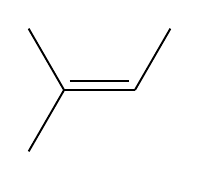
\begin{tikzpicture}[scale=0.9, line width=0.7pt]
  \draw (0,0) -- (1,0);
  \draw (0.08,0.13) -- (0.92,0.13);
  \draw (0,0) -- (-0.5,0.866);
  \draw (0,0) -- (-0.5,-0.866);
  \draw (1,0) -- (1.5,0.866);
\end{tikzpicture}\\
a) X
\end{minipage}\hfill
\begin{minipage}[t]{0.23\textwidth}\centering
\begin{tikzpicture}[scale=0.9, line width=0.7pt]
  \draw (-1,0) -- (1,0);
  \draw (0,0) -- (0,1);
  \draw (0,0) -- (0,-0.6);
  \node[anchor=north] at (0,-0.6) {Br};
  \draw (1,0) -- (1.5,-0.866);
\end{tikzpicture}\\
b) Z
\end{minipage}\hfill
\begin{minipage}[t]{0.23\textwidth}\centering
\begin{tikzpicture}[scale=0.9, line width=0.7pt]
  \draw (0,0) -- (0.866,0.5) -- (1.732,0) -- (2.598,0.5);
  \draw (1.732,0) -- (1.732,-1);
  \draw (0.866,0.5) -- (0.866,1.0);
  \node[anchor=south] at (0.866,1.0) {Br};
\end{tikzpicture}\\
c) G (racêmico)
\end{minipage}\hfill
\begin{minipage}[t]{0.23\textwidth}\centering
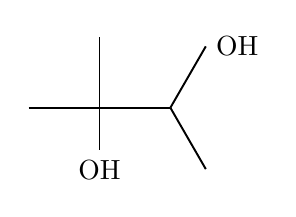
\begin{tikzpicture}[scale=0.9, line width=0.7pt]
  \draw (-1,0) -- (1,0);
  \draw (0,0) -- (0,1);
  \draw (0,0) -- (0,-0.6);
  \node[anchor=north] at (0,-0.6) {OH};
  \draw (1,0) -- (1.5,0.866);
  \node[anchor=west] at (1.5,0.866) {OH};
  \draw (1,0) -- (1.5,-0.866);
\end{tikzpicture}\\
d) J (racêmico)
\end{minipage}

\textbf{Conferências e sensibilidade.} Os balanços fecham em todas as etapas. Z e G são regiosisômeros; Z é aquiral; G e J são racêmicos. Se X fosse o 2-metilbut-1-eno, Z não mudaria (mesmo carbocátion terciário), G seria o 1-bromo-2-metilbutano, $\mathrm{BrCH_2{-}CH(CH_3){-}CH_2CH_3}$, e J seria o 2-metilbutano-1,2-diol, $\mathrm{HOCH_2{-}C(OH)(CH_3){-}CH_2CH_3}$. Logo, c) e d) dependem da escolha de X.

ANSWER: a) X = 2-metilbut-2-eno, $(\mathrm{CH_3})_2\mathrm{C{=}CH{-}CH_3}$; b) Z = 2-bromo-2-metilbutano, $(\mathrm{CH_3})_2\mathrm{CBr{-}CH_2CH_3}$; c) G = 2-bromo-3-metilbutano, $(\mathrm{CH_3})_2\mathrm{CH{-}CHBr{-}CH_3}$ (mistura racêmica); d) J = 2-metilbutano-2,3-diol, $(\mathrm{CH_3})_2\mathrm{C(OH){-}CH(OH){-}CH_3}$ (mistura racêmica)%
\newpage%
\section*{Questão 4}

\section*{Solução}

\textbf{Hipóteses.}
\begin{enumerate}
\item Os sais são totalmente dissolvidos e dissociados (eletrólitos fortes), sem hidrólise, precipitação ou complexação dos íons.
\item A parcela não pura de cada amostra é inerte: não libera íons e não altera as quantidades de matéria. Essa parcela é de 10\% em QX e TX$_3$ e de $(100-P)$\% em RX$_2$.
\item A concentração total de cátions é a soma das concentrações molares: $[\mathrm{Q}^{+}]+[\mathrm{R}^{2+}]+[\mathrm{T}^{3+}]=2\ \mathrm{mol\cdot L^{-1}}$. Não se trata de soma de cargas.
\item A proporção molar $6:3:1$ refere-se a quantidades de matéria, em mol.
\item O volume final da solução é $V=500\ \mathrm{mL}=0{,}5\ \mathrm{L}$.
\item X é um ânion monovalente, $\mathrm{X}^{-}$, coerente com as fórmulas QX, RX$_2$ e TX$_3$ e com as cargas $+1$, $+2$ e $+3$ dos cátions.
\end{enumerate}

\textbf{1. Quantidade total de cátions.}
\[
n_{\mathrm{total}}=[\text{cátions}]\cdot V=2\ \mathrm{mol\cdot L^{-1}}\cdot 0{,}5\ \mathrm{L}=1{,}0\ \mathrm{mol}
\]

\textbf{2. Quantidade de cada cátion.} A proporção $6:3:1$ tem $6+3+1=10$ partes. Cada parte vale $1{,}0/10=0{,}1\ \mathrm{mol}$:
\[
n(\mathrm{Q}^{+})=6\cdot 0{,}1=0{,}6\ \mathrm{mol}\qquad n(\mathrm{R}^{2+})=3\cdot 0{,}1=0{,}3\ \mathrm{mol}\qquad n(\mathrm{T}^{3+})=1\cdot 0{,}1=0{,}1\ \mathrm{mol}
\]
Conferência: $0{,}6+0{,}3+0{,}1=1{,}0\ \mathrm{mol}$, valor obtido no passo 1.

\textbf{a) Massa de QX.} Cada fórmula QX fornece um íon Q$^{+}$. A massa pura necessária é $0{,}6\ \mathrm{mol}\cdot 60\ \mathrm{g\cdot mol^{-1}}=36\ \mathrm{g}$. Com pureza de 90\%, a massa da amostra satisfaz
\[
0{,}90\cdot m=36\ \mathrm{g}\;\Rightarrow\; m=\frac{36}{0{,}90}=40\ \mathrm{g}
\]
Os 4 g restantes são impurezas.

\textbf{b) Pureza do RX$_2$.} Cada fórmula RX$_2$ fornece um íon R$^{2+}$. A massa pura necessária é $0{,}3\ \mathrm{mol}\cdot 150\ \mathrm{g\cdot mol^{-1}}=45\ \mathrm{g}$. Com 60 g de amostra,
\[
\frac{P}{100}\cdot 60\ \mathrm{g}=45\ \mathrm{g}\;\Rightarrow\; P=75
\]
Logo, a pureza é 75\%. Conferência: $45\ \mathrm{g}/150\ \mathrm{g\cdot mol^{-1}}=0{,}3\ \mathrm{mol}$.

\textbf{c) Massa molar do TX$_3$.} A massa pura é $0{,}90\cdot 20\ \mathrm{g}=18\ \mathrm{g}$. Ela contém $0{,}1\ \mathrm{mol}$ de T$^{3+}$, pois cada fórmula fornece um íon T$^{3+}$:
\[
MM=\frac{18\ \mathrm{g}}{0{,}1\ \mathrm{mol}}=180\ \mathrm{g\cdot mol^{-1}}
\]

\textbf{d) Concentração de X$^{-}$.} O número de íons X$^{-}$ liberados por fórmula é o subscrito de X: QX libera 1, RX$_2$ libera 2 e TX$_3$ libera 3. Como os sais se dissociam totalmente,
\[
n(\mathrm{X}^{-})=1\cdot 0{,}6+2\cdot 0{,}3+3\cdot 0{,}1=0{,}6+0{,}6+0{,}3=1{,}5\ \mathrm{mol}
\]
\[
[\mathrm{X}^{-}]=\frac{1{,}5\ \mathrm{mol}}{0{,}5\ \mathrm{L}}=3{,}0\ \mathrm{mol\cdot L^{-1}}
\]

\textbf{Conferências.}
\begin{itemize}
\item Eletroneutralidade: a carga positiva total é $0{,}6\cdot 1+0{,}3\cdot 2+0{,}1\cdot 3=1{,}5\ \mathrm{mol}$ de carga. Ela é igual à carga negativa de $1{,}5\ \mathrm{mol}$ de X$^{-}$.
\item Pelas concentrações dos cátions, $[\mathrm{Q}^{+}]=1{,}2$, $[\mathrm{R}^{2+}]=0{,}6$ e $[\mathrm{T}^{3+}]=0{,}2\ \mathrm{mol\cdot L^{-1}}$. Então $[\mathrm{X}^{-}]=1\cdot 1{,}2+2\cdot 0{,}6+3\cdot 0{,}2=3{,}0\ \mathrm{mol\cdot L^{-1}}$.
\item Ordem de grandeza: a carga média por cátion é $1{,}5/1{,}0=1{,}5$. Logo $[\mathrm{X}^{-}]=1{,}5\cdot 2{,}0=3{,}0\ \mathrm{mol\cdot L^{-1}}$.
\item Coerência das massas: $m=36/0{,}90$ é maior que 36 g, como esperado para amostra impura. A pureza $P=75\%$ está entre 0 e 100\%, e a massa molar $MM=180\ \mathrm{g\cdot mol^{-1}}$ é positiva.
\end{itemize}

ANSWER: a) $m = 40\ \mathrm{g}$; b) P = 75\%; c) $MM = 180\ \mathrm{g\cdot mol^{-1}}$; d) $[\mathrm{X}^{-}] = 3{,}0\ \mathrm{mol\cdot L^{-1}}$.%
\newpage%
\section*{Questão 5}

\section*{Solução}

\textbf{Convenções.} Substância simples tem NOX $0$ (N$_2$). Em uma espécie, a soma dos NOX dos átomos é igual à carga. O oxigênio tem NOX $-2$ (não há peróxidos nesta questão). O hidrogênio ligado a N ou O, que são mais eletronegativos, tem NOX $+1$. Redução é diminuição do NOX (ganho de elétrons); oxidação é aumento do NOX (perda de elétrons).

\textbf{a) Resposta:} $\mathrm{N_2 + 8\,H^{+} + 6\,e^{-} \longrightarrow 2\,NH_4^{+}}$

\emph{Escolha do produto.} Reduzir o N$_2$ (NOX $0$) exige um produto com NOX menor que $0$. Pelo item b), NH$_4^+$ tem NOX $-3$. As demais espécies listadas têm NOX positivo: NO ($+2$), NO$_2^-$ ($+3$), NO$_3^-$ ($+5$) e N$_2$O (média $+1$). Logo, NH$_4^+$ é o único produto possível. Em meio ácido, o nitrogênio reduzido é formado como NH$_3$, que é protonado a NH$_4^+$. Como NH$_4^+$ é a espécie listada, ela é o produto da semirreação.

\emph{Balanceamento.} Não há oxigênio na reação, então não entra H$_2$O. O meio é ácido, então o hidrogênio é ajustado com H$^+$.
\begin{enumerate}
\item N: há $2$ átomos de N em cada lado, com coeficiente $2$ para NH$_4^+$.
\item H: o produto tem $8$ H; somamos $8\,\mathrm{H^+}$ ao reagente.
\item Carga: o reagente passa a ter carga $+8$ e o produto tem carga $+2$. Somamos $6\,\mathrm{e^-}$ ao reagente, de modo que $+8-6=+2$.
\item Conferência: N $2=2$; H $8=8$; carga $+2=+2$. Os elétrons conferem com a variação de NOX: cada N vai de $0$ a $-3$ e ganha $3\,\mathrm{e^-}$, logo $2$ N ganham $6\,\mathrm{e^-}$.
\end{enumerate}

\textbf{b) Resposta:} NO: $+2$; NO$_3^-$: $+5$; N$_2$: $0$; NH$_4^+$: $-3$; NO$_2^-$: $+3$; N$_2$O (média): $+1$.

\emph{Cálculos}, com $x$ o NOX do N em cada espécie:
\begin{itemize}
\item NO: $x-2=0$, logo $x=+2$.
\item NO$_3^-$: $x-6=-1$, logo $x=+5$.
\item N$_2$: substância simples, NOX $0$.
\item NH$_4^+$: $x+4=+1$, logo $x=-3$.
\item NO$_2^-$: $x-4=-1$, logo $x=+3$.
\item N$_2$O: os dois N não são equivalentes, e a regra fixa apenas a soma. Com $\bar{x}$ a média, $2\bar{x}-2=0$, logo $\bar{x}=+1$.
\end{itemize}
Os NOX individuais de N$_2$O dependem da estrutura de Lewis. Por exemplo, $\mathrm{N\equiv N^{+}-O^{-}}$ dá $0$ e $+2$, e $\mathrm{N^{-}=N^{+}=O}$ dá $-1$ e $+3$. Nas duas, a soma é $+2$. A média, $+1$, é a grandeza pedida e não depende da estrutura.

\textbf{c) Resposta:} $\mathrm{N_2 \rightarrow NH_4^{+} \rightarrow NO_2^{-} \rightarrow NO_3^{-} \rightarrow NO_2^{-} \rightarrow NO \rightarrow N_2O}$, com a desnitrificação parcial terminando em N$_2$O.

Verificamos o sentido da variação do NOX em cada processo.
\begin{enumerate}
\item \emph{Fixação biológica do N$_2$} (bactérias diazotróficas, com a enzima nitrogenase): N$_2$ ($0$) $\rightarrow$ NH$_4^+$ ($-3$). O NOX diminui, logo é redução. A semirreação da letra a) representa apenas o balanço formal de NOX e de elétrons, não a estequiometria da enzima. A nitrogenase consome $8\,\mathrm{e^-}$ por N$_2$: $6$ para formar $2$ NH$_3$ e $2$ para formar H$_2$, que é produzido obrigatoriamente. Ela também consome $16$ ATP por N$_2$. Em meio aquoso, o NH$_3$ liberado é protonado a NH$_4^+$.
\item \emph{Nitrificação} (solos aerados, com O$_2$ como aceptor de elétrons, em duas etapas feitas por bactérias quimiolitoautotróficas):
\begin{itemize}
\item Nitrosomonas: $\mathrm{NH_4^{+} + \tfrac{3}{2}\,O_2 \longrightarrow NO_2^{-} + 2\,H^{+} + H_2O}$ (NOX $-3 \rightarrow +3$, com perda de $6\,\mathrm{e^-}$ pelo N).
\item Nitrobacter: $\mathrm{NO_2^{-} + \tfrac{1}{2}\,O_2 \longrightarrow NO_3^{-}}$ (NOX $+3 \rightarrow +5$, com perda de $2\,\mathrm{e^-}$ pelo N).
\end{itemize}
Ambas são oxidações.
\item \emph{Desnitrificação parcial} (baixo O$_2$; bactérias usam NO$_3^-$ como aceptor final de elétrons): NO$_3^-$ ($+5$) $\rightarrow$ NO$_2^-$ ($+3$) $\rightarrow$ NO ($+2$) $\rightarrow$ N$_2$O ($+1$). Cada etapa diminui o NOX, logo são reduções. A sequência para em N$_2$O porque o processo é parcial, ou seja, a redução não chega a N$_2$.
\end{enumerate}

Juntando as etapas na ordem fixação, nitrificação e desnitrificação:
\[
\mathrm{N_2 \rightarrow NH_4^{+} \rightarrow NO_2^{-} \rightarrow NO_3^{-} \rightarrow NO_2^{-} \rightarrow NO \rightarrow N_2O}
\]
NOX: $0 \rightarrow -3 \rightarrow +3 \rightarrow +5 \rightarrow +3 \rightarrow +2 \rightarrow +1$. Há redução na fixação, oxidações na nitrificação e reduções na desnitrificação. As seis espécies fornecidas aparecem, e NO$_2^-$ aparece duas vezes, como o enunciado permite.

\emph{Sobre a palavra "parcial".} O enunciado qualifica a desnitrificação como parcial, e o item c) refere-se a esse mesmo processo. Por isso adotamos a sequência que para em N$_2$O, que é o produto da redução incompleta e é liberado para a atmosfera. Essa sequência é compatível com o ciclo, pois é um trecho dele, e o ciclo não precisa ser fechado. Se a desnitrificação fosse completa, o que equivale a ignorar o qualificador, a sequência continuaria com N$_2$O ($+1$) $\rightarrow$ N$_2$ ($0$), fechando o ciclo no N$_2$ inicial: $\mathrm{N_2 \rightarrow NH_4^{+} \rightarrow NO_2^{-} \rightarrow NO_3^{-} \rightarrow NO_2^{-} \rightarrow NO \rightarrow N_2O \rightarrow N_2}$. Essa leitura alternativa usa as mesmas espécies e não muda os itens a) e b).

ANSWER: a) $\mathrm{N_2 + 8\,H^{+} + 6\,e^{-} \longrightarrow 2\,NH_4^{+}}$; b) NO: $+2$; NO$_3^-$: $+5$; N$_2$: $0$; NH$_4^+$: $-3$; NO$_2^-$: $+3$; N$_2$O (média): $+1$; c) $\mathrm{N_2 \rightarrow NH_4^{+} \rightarrow NO_2^{-} \rightarrow NO_3^{-} \rightarrow NO_2^{-} \rightarrow NO \rightarrow N_2O}$ (desnitrificação parcial; se a desnitrificação for completa, a sequência se prolonga até N$_2$)%
\newpage%
\section*{Questão 6}

\section*{Solução}

Escolho três reações: (1) lítio com água; (2) reação global do metano com vapor d'água, que combina reforma a vapor e deslocamento gás-água; (3) pirólise do metano.

\textbf{Hipóteses.}
\begin{itemize}
\item Gases ideais; $\Delta H^\circ$ e $\Delta S^\circ$ constantes no intervalo de temperatura considerado.
\item Estado padrão: 1 bar para gases, atividade unitária para solutos e sólido na forma mais estável. A espontaneidade é avaliada nesse estado.
\item ``Reação completa'': consumo total do reagente limitante segundo a estequiometria, sem considerar equilíbrio, cinética ou reações paralelas. É uma idealização, discutida no item iii da reação 2.
\item Os dados abaixo (298 K, 1 bar) e os potenciais padrão são valores tabelados usuais, não fornecidos na prova. Servem apenas à verificação termodinâmica do item iii. O item iv não depende deles.
\end{itemize}

\begin{center}
\begin{tabular}{lcc}
Substância & $\Delta H_f^\circ$ ($\mathrm{kJ\,mol^{-1}}$) & $S^\circ$ ($\mathrm{J\,mol^{-1}\,K^{-1}}$) \\
\hline
$\mathrm{H_2O}(\ell)$ & $-285{,}8$ & $69{,}9$ \\
$\mathrm{H_2O}(g)$ & $-241{,}8$ & $188{,}8$ \\
$\mathrm{CH_4}(g)$ & $-74{,}8$ & $186{,}3$ \\
$\mathrm{CO}(g)$ & $-110{,}5$ & $197{,}7$ \\
$\mathrm{CO_2}(g)$ & $-393{,}5$ & $213{,}8$ \\
$\mathrm{H_2}(g)$ & $0$ & $130{,}7$ \\
$\mathrm{C}(\text{grafite}, s)$ & $0$ & $5{,}7$ \\
$\mathrm{LiOH}(aq)$ & $-508{,}5$ & -- \\
\end{tabular}
\end{center}

Potenciais padrão tabelados: $E^\circ(\mathrm{Li^+/Li}) = -3{,}04$ V e $E^\circ(\mathrm{H_2O/H_2}) = -0{,}83$ V (meio básico, $[\mathrm{OH^-}] = 1$ mol/L).

\textbf{Reação 1: lítio com água.}

\textbf{i)} Reagentes: Li($s$) e H$_2$O($\ell$). Produtos: LiOH($aq$) e H$_2$($g$).

\textbf{ii)}
\[ 2\,\mathrm{Li}(s) + 2\,\mathrm{H_2O}(\ell) \rightarrow 2\,\mathrm{LiOH}(aq) + \mathrm{H_2}(g) \]
Li: $0 \rightarrow +1$ (cede $1\,e^-$ por átomo). H da água: $+1 \rightarrow 0$ (recebe $1\,e^-$ por H). Cada H$_2$ exige $2\,e^-$, logo 2 Li. Semirreações: $\mathrm{Li \rightarrow Li^+ + e^-}$ (multiplicada por 2) e $\mathrm{2\,H_2O + 2\,e^- \rightarrow H_2 + 2\,OH^-}$. Conferência: Li $2=2$; O $2=2$; H $4=2+2$.

\textbf{iii)} Interpreto ``condições básicas'' como condições essenciais. São necessárias água líquida (0 a $100\,^\circ$C, 1 atm) e superfície de Li limpa, pois a película de Li$_2$O/LiOH formada no ar retarda a reação. Não há necessidade de aquecimento nem de catalisador: a reação ocorre a $25\,^\circ$C, com velocidade moderada (mais lenta que com Na e K). O meio final é básico, mas isso é produto da reação. Verificação termodinâmica:
\[ E^\circ_{\text{cél}} = E^\circ_{\text{cat}} - E^\circ_{\text{an}} = (-0{,}83) - (-3{,}04) = +2{,}21\ \mathrm{V} > 0 \]
\[ \Delta G^\circ = -nFE^\circ = -2\,(9{,}65\times 10^4)(2{,}21) \approx -4{,}27\times 10^5\ \mathrm{J} \approx -427\ \mathrm{kJ} \]
com $n = 2$, pela equação do item ii. Pela entalpia, $\Delta H^\circ = 2(-508{,}5) - 2(-285{,}8) \approx -445\ \mathrm{kJ}$. A reação é espontânea e exotérmica. A solução final é básica, pois LiOH é base forte.

\textbf{Reação 2: reação global do metano com vapor d'água (reforma a vapor e deslocamento gás-água).}

\textbf{i)} Reagentes: CH$_4$($g$) e H$_2$O($g$), pois a reação ocorre acima de $100\,^\circ$C. Produtos: CO$_2$($g$) e H$_2$($g$).

\textbf{ii)}
\[ \mathrm{CH_4}(g) + 2\,\mathrm{H_2O}(g) \rightarrow \mathrm{CO_2}(g) + 4\,\mathrm{H_2}(g) \]
É a soma de duas etapas, com CO como intermediário. Reforma:
\[ \mathrm{CH_4}(g) + \mathrm{H_2O}(g) \rightarrow \mathrm{CO}(g) + 3\,\mathrm{H_2}(g) \]
Deslocamento gás-água:
\[ \mathrm{CO}(g) + \mathrm{H_2O}(g) \rightarrow \mathrm{CO_2}(g) + \mathrm{H_2}(g) \]
Conferência: C $1=1$; O $2=2$; H $4+4=8=4\cdot 2$. Redox: C vai de $-4$ a $+4$ (cede $8\,e^-$); os 8 H vão de $+1$ a $0$ (recebem $8\,e^-$).

\textbf{iii)} Condições da prática industrial:
\begin{itemize}
\item Reforma (endotérmica): $800$ a $900\,^\circ$C, catalisador Ni/Al$_2$O$_3$, razão H$_2$O:CH$_4$ de 2,5 a 3,5 (mínimo estequiométrico 2). O excesso de vapor reduz a deposição de carbono. Baixa pressão favorece o equilíbrio ($\Delta n_{\mathrm{gas}} = 5 - 3 = +2$), mas a indústria opera tipicamente a 15 a 30 bar por razões econômicas, como o volume dos equipamentos e o uso posterior do gás. A pressão moderada é o compromisso.
\item Deslocamento: $\Delta H^\circ = -41{,}2\ \mathrm{kJ\,mol^{-1}}$ e $\Delta S^\circ = -42{,}0\ \mathrm{J\,K^{-1}\,mol^{-1}}$. Logo $\Delta G^\circ < 0$ só para $T < 981\ \mathrm{K}$ ($708\,^\circ$C). Como $K \approx 2\times 10^2$ a 200 $^\circ$C, $K \approx 10$ a 400 $^\circ$C e $K \approx 0{,}9$ a 1000 K, a conversão de CO a CO$_2$ é favorecida em temperatura baixa. Por isso o deslocamento é feito em duas etapas, após o resfriamento do gás: cerca de 350 $^\circ$C (catalisador Fe$_2$O$_3$/Cr$_2$O$_3$) e 200 a 250 $^\circ$C (Cu/ZnO).
\end{itemize}

Verificação termodinâmica da equação global:
\[ \Delta H^\circ = \left[-393{,}5\right] - \left[-74{,}8 + 2(-241{,}8)\right] = +164{,}9\ \mathrm{kJ\,mol^{-1}} \]
\[ \Delta S^\circ = \left[213{,}8 + 4(130{,}7)\right] - \left[186{,}3 + 2(188{,}8)\right] = +172{,}7\ \mathrm{J\,K^{-1}\,mol^{-1}} \]
\[ \Delta G^\circ < 0 \Leftrightarrow T > \frac{164{,}9}{0{,}1727} \approx 955\ \mathrm{K}\ (\approx 682\,^\circ\mathrm{C}) \]
A 298 K, $\Delta G^\circ \approx +113$ kJ, logo não é espontânea. A 1000 K, $\Delta G^\circ \approx -8$ kJ e $K \approx 2{,}6$, produto de $K_{\text{reforma}} \approx 2{,}8$ e $K_{\text{desl}} \approx 0{,}9$. Com $K \approx 2{,}6$, o equilíbrio global a 1000 K não é total e ainda contém CO. Por isso ``completa'' é idealização, que exige o deslocamento em temperatura baixa.

\textbf{Reação 3: pirólise do metano.}

\textbf{i)} Reagente: CH$_4$($g$). Produtos: C($\text{grafite}$, $s$) e H$_2$($g$). O grafite é a forma sólida mais estável do carbono a 1 bar.

\textbf{ii)}
\[ \mathrm{CH_4}(g) \rightarrow \mathrm{C}(\text{grafite}, s) + 2\,\mathrm{H_2}(g) \]
C: $-4 \rightarrow 0$ (cede $4\,e^-$). Quatro H: $+1 \rightarrow 0$ (recebem $4\,e^-$). Conferência: C $1=1$; H $4=2\cdot 2$.

\textbf{iii)} Temperatura elevada:
\[ \Delta H^\circ = 0 - (-74{,}8) = +74{,}8\ \mathrm{kJ\,mol^{-1}}, \qquad \Delta S^\circ = \left[5{,}7 + 2(130{,}7)\right] - 186{,}3 = +80{,}8\ \mathrm{J\,K^{-1}\,mol^{-1}} \]
\[ \Delta G^\circ < 0 \Leftrightarrow T > \frac{74{,}8}{0{,}0808} \approx 926\ \mathrm{K}\ (\approx 653\,^\circ\mathrm{C}) \]
A 298 K, $\Delta G^\circ \approx +51$ kJ, logo não ocorre à temperatura ambiente. Na prática, a cinética exige cerca de 1000 $^\circ$C na pirólise térmica, e catalisadores metálicos (Ni, Fe) reduzem essa exigência. Baixa pressão favorece a reação ($\Delta n_{\mathrm{gas}} = 2 - 1 = +1$). Deve-se excluir O$_2$, que causaria combustão.

\textbf{iv) Rendimento de H$_2$ por mol de reagente, reação completa.}

Base adotada: mol de H$_2$ formado dividido pelo total de mols de reagentes consumidos na equação balanceada. As três reações têm conjuntos de reagentes diferentes. Esta é a única base que se aplica às três ao mesmo tempo, sem privilegiar uma espécie. Por mol de CH$_4$, a reação 1 não se aplica. Por mol de H$_2$O, a reação 3 não se aplica. As outras bases estão na tabela.

\begin{center}
\begin{tabular}{lccccc}
Reação & Reagentes (mol) & H$_2$ (mol) & Por mol de reagente total & Por mol de CH$_4$ & Por mol de H$_2$O \\
\hline
1: $2\,\mathrm{Li} + 2\,\mathrm{H_2O}$ & 4 & 1 & 0,25 & -- & 0,5 \\
2: $\mathrm{CH_4} + 2\,\mathrm{H_2O}$ & 3 & 4 & 1,33 & 4 & 2 \\
3: $\mathrm{CH_4}$ & 1 & 2 & 2,0 & 2 & -- \\
\end{tabular}
\end{center}

Por mol de Li, só a reação 1 se aplica, com 0,5 mol de H$_2$.

\textbf{Cota geral.} Cada H$_2$ tem 2 átomos de H, que só podem vir dos reagentes. Logo $2\,n_{\mathrm{H_2}} \leq 4\,n_{\mathrm{CH_4}} + 2\,n_{\mathrm{H_2O}}$, ou seja, $n_{\mathrm{H_2}} \leq 2\,n_{\mathrm{CH_4}} + n_{\mathrm{H_2O}}$. Dividindo pelo total de mols de reagentes:
\[ \frac{n_{\mathrm{H_2}}}{n_{\text{reag}}} \leq \frac{2\,n_{\mathrm{CH_4}} + n_{\mathrm{H_2O}}}{n_{\mathrm{CH_4}} + n_{\mathrm{H_2O}} + n_{\mathrm{Li}}} \leq 2 \]
A segunda desigualdade equivale a $n_{\mathrm{H_2O}} + 2\,n_{\mathrm{Li}} \geq 0$, com igualdade apenas se não houver H$_2$O nem Li. Assim, 2 mol de H$_2$ por mol de reagente total é o máximo possível com esses reagentes, atingido só pela pirólise do CH$_4$ puro.

\textbf{Conclusão.} Pela base de reagente total, a reação 3 rende 2,0 mol de H$_2$ por mol de reagente, o máximo possível. A reação 2 rende 1,33 (1,5 se o CO não for convertido em CO$_2$). A conclusão depende da base. Por mol de CH$_4$, a reação 2 vence (4 contra 2). Por mol de H$_2$O, a reação 2 também vence (2 contra 0,5). Adoto a base de reagente total, declarada acima, e a resposta fica explícita na linha final.

ANSWER: pirólise do metano, $\mathrm{CH_4}(g) \rightarrow \mathrm{C}(\text{grafite}, s) + 2\,\mathrm{H_2}(g)$, com 2,0 mol de H$_2$ por mol de reagente total (base adotada; por mol de CH$_4$, a reforma rende mais: 4 contra 2)%
\newpage%
\section*{Questão 7}

\section*{Solução}

\textbf{Convenções.} Todas as espécies estão em seus estados padrão a 298 K: líquidos puros e O$_2$ gasoso a 1 bar, com $\Delta H^\circ_f(\text{O}_2,\,g)=0$ por definição. Dados que não constam da prova são marcados com \textbf{(ext.)} e não entram em nenhum cálculo numérico.

\textbf{a) Rota sintética em duas etapas}

\textit{Etapa 1: oxidação completa do etanol a ácido acético.}
\[
\text{CH}_3\text{CH}_2\text{OH}(\ell) + \text{O}_2(g) \longrightarrow \text{CH}_3\text{COOH}(\ell) + \text{H}_2\text{O}(\ell)
\]
Balanço atômico: C ($2=2$), H ($6=4+2$) e O ($1+2=2+1$). Balanço eletrônico: o carbono do grupo CH$_2$OH passa do nox $-1$ para $+3$, cedendo $4$ elétrons por etanol; cada O$_2$ recebe $4$ elétrons, pois cada átomo de O vai de $0$ a $-2$. A proporção 1:1 é consistente com isso.

Condições possíveis:
\begin{itemize}
\item Via biológica (vinagre): O$_2$ do ar, meio aquoso aerado, catálise por bactérias acéticas do gênero \textit{Acetobacter}, a temperatura ambiente de cerca de $25$ a $30\,^\circ$C \textbf{(ext.)}.
\item Via laboratorial: dicromato de potássio em H$_2$SO$_4$ diluído, em excesso, sob aquecimento e refluxo:
\[
3\,\text{CH}_3\text{CH}_2\text{OH} + 2\,\text{K}_2\text{Cr}_2\text{O}_7 + 8\,\text{H}_2\text{SO}_4 \longrightarrow 3\,\text{CH}_3\text{COOH} + 2\,\text{Cr}_2(\text{SO}_4)_3 + 2\,\text{K}_2\text{SO}_4 + 11\,\text{H}_2\text{O}
\]
Balanço eletrônico: 3 etanóis cedem $3\times 4=12$ elétrons; 2 dicromatos contêm 4 Cr($+6$), que passam a Cr($+3$) e recebem $4\times 3=12$ elétrons. Os átomos de K, Cr, S, C, H e O também conferem.
\end{itemize}

Justificativas:
\begin{itemize}
\item O refluxo evita a perda do acetaldeído (p.e. cerca de $20\,^\circ$C \textbf{(ext.)}) por destilação, mantendo-o no meio até a oxidação a ácido.
\item A oxidação completa exige oxidante forte ou o sistema enzimático. Oxidantes brandos, como PCC ou cobre aquecido, param no aldeído.
\item O meio ácido é necessário para o dicromato: em meio básico ele se converte em cromato, oxidante bem mais fraco.
\end{itemize}

\textit{Etapa 2: esterificação de Fischer.}
\[
\text{CH}_3\text{COOH}(\ell) + \text{CH}_3\text{CH}_2\text{OH}(\ell) \rightleftharpoons \text{CH}_3\text{COOCH}_2\text{CH}_3(\ell) + \text{H}_2\text{O}(\ell)
\]
Condições:
\begin{itemize}
\item Catalisador: H$_2$SO$_4$ concentrado, em pequena quantidade. O ácido protona a carbonila, tornando o carbono mais eletrófilo para o ataque do etanol. O H$_2$SO$_4$ concentrado também absorve água, o que desloca o equilíbrio.
\item A reação é reversível. Pelo princípio de Le Châtelier, o equilíbrio se desloca com etanol em excesso ou com a remoção da água, por exemplo por arraste azeotrópico com tolueno ou benzeno em aparelho de Dean-Stark.
\item A temperatura de refluxo depende do método. Com etanol em excesso, a mistura ferve perto de $78\,^\circ$C \textbf{(ext.)}, a temperatura de ebulição do etanol. Com Dean-Stark, a mistura ferve em temperatura mais alta, próxima da do arrastador \textbf{(ext.)}.
\item O meio deve ser ácido. Em meio básico (ex.: NaOH) o éster sofreria saponificação, hidrólise irreversível a acetato e etanol, o inverso do pretendido.
\end{itemize}

Conferência: somando uma vez a etapa 1 e uma vez a etapa 2, o ácido acético é intermediário e se cancela:
\[
2\,\text{CH}_3\text{CH}_2\text{OH}(\ell) + \text{O}_2(g) \longrightarrow \text{CH}_3\text{COOCH}_2\text{CH}_3(\ell) + 2\,\text{H}_2\text{O}(\ell)
\]
Esta é exatamente a reação global do enunciado. Logo, a rota com O$_2$ é a consistente com o enunciado; a via com dicromato é alternativa de laboratório.

\textbf{b) Variação de entalpia padrão}

A entalpia é função de estado. Pela lei de Hess, na forma das entalpias de formação,
\[
\Delta H^\circ_r = \sum n_{\text{prod}}\,\Delta H^\circ_f - \sum n_{\text{reag}}\,\Delta H^\circ_f
\]
\begin{align*}
\sum n_{\text{prod}}\,\Delta H^\circ_f &= 1\,(-480{,}0) + 2\,(-285{,}8) = -1051{,}6\ \text{kJ} \\
\sum n_{\text{reag}}\,\Delta H^\circ_f &= 2\,(-277{,}7) + 1\,(0{,}0) = -555{,}4\ \text{kJ} \\
\Delta H^\circ_r &= -1051{,}6 - (-555{,}4) = -496{,}2\ \text{kJ}
\end{align*}
O valor refere-se à reação como escrita, com 2 mol de etanol e 1 mol de O$_2$ consumidos e 1 mol de éster e 2 mol de água formados. O sinal negativo indica reação exotérmica. Por mol de etanol consumido, $\Delta H^\circ = -248{,}1\ \text{kJ}\cdot\text{mol}^{-1}$.

\textbf{c) Variação de entropia padrão}

A entropia também é função de estado, e os valores tabelados são absolutos (terceira lei). Por isso, a variação é a diferença entre as somas ponderadas das entropias molares:
\[
\Delta S^\circ_r = \sum n_{\text{prod}}\,S^\circ_m - \sum n_{\text{reag}}\,S^\circ_m
\]
\begin{align*}
\sum n_{\text{prod}}\,S^\circ_m &= 259{,}4 + 2\,(69{,}9) = 399{,}2\ \text{J}\cdot\text{K}^{-1} \\
\sum n_{\text{reag}}\,S^\circ_m &= 2\,(160{,}7) + 205{,}0 = 526{,}4\ \text{J}\cdot\text{K}^{-1} \\
\Delta S^\circ_r &= 399{,}2 - 526{,}4 = -127{,}2\ \text{J}\cdot\text{K}^{-1}
\end{align*}
Para interpretar, separa-se a contribuição das fases condensadas da do gás:
\begin{align*}
\Delta S^\circ_r &= \underbrace{\left[259{,}4 + 2\,(69{,}9) - 2\,(160{,}7)\right]}_{\text{fases condensadas}} \;\underbrace{-\,205{,}0}_{\text{O}_2\,(g)} \\
&= (+77{,}8) - 205{,}0 = -127{,}2\ \text{J}\cdot\text{K}^{-1}
\end{align*}
A parcela condensada é positiva porque o número de mols de líquidos sobe de 2 (etanol) para 3 (éster e 2 água). A saída de 1 mol de O$_2$ gasoso, com entropia alta, remove $205{,}0\ \text{J}\cdot\text{K}^{-1}$ e domina o resultado. O sinal negativo é coerente com $\Delta n_{\text{gás}}=-1$.

\textbf{d) Variação de energia de Gibbs padrão a 298 K}
\[
\Delta G^\circ_r = \Delta H^\circ_r - T\,\Delta S^\circ_r
\]
Como todos os dados são a 298 K, a relação é aplicada diretamente nessa temperatura. Para coerência de unidades, $\Delta S^\circ_r = -0{,}1272\ \text{kJ}\cdot\text{K}^{-1}$:
\begin{align*}
T\,\Delta S^\circ_r &= 298\ \text{K}\times(-0{,}1272\ \text{kJ}\cdot\text{K}^{-1}) = -37{,}9\ \text{kJ} \\
\Delta G^\circ_r &= -496{,}2 - (-37{,}9) = -458{,}3\ \text{kJ}
\end{align*}
Como $\Delta G^\circ_r<0$, a reação é espontânea a 298 K nas condições padrão. Isso não informa a velocidade: sem catalisador, a oxidação do etanol pelo O$_2$ do ar é muito lenta a 298 K, e a reação só se observa com catálise. O termo $-T\,\Delta S^\circ_r = +37{,}9\ \text{kJ}$ se opõe à reação, mas equivale a cerca de $7{,}6\%$ de $|\Delta H^\circ_r|$. Pela extrapolação linear, $\Delta G^\circ_r$ só se anularia em $T\approx 3{,}9\times 10^{3}\ \text{K}$, temperatura sem aplicação prática, pois as substâncias mudam de fase muito antes \textbf{(ext.)}.

ANSWER: a) Etapa 1: $\text{CH}_3\text{CH}_2\text{OH}(\ell) + \text{O}_2(g) \longrightarrow \text{CH}_3\text{COOH}(\ell) + \text{H}_2\text{O}(\ell)$ (catálise por \textit{Acetobacter} em meio aerado; alternativa de laboratório: $\text{K}_2\text{Cr}_2\text{O}_7$/$\text{H}_2\text{SO}_4$ com refluxo). Etapa 2: $\text{CH}_3\text{COOH}(\ell) + \text{CH}_3\text{CH}_2\text{OH}(\ell) \rightleftharpoons \text{CH}_3\text{COOCH}_2\text{CH}_3(\ell) + \text{H}_2\text{O}(\ell)$ (H$_2$SO$_4$ concentrado, catálise ácida, remoção de água). b) $\Delta H^\circ_r = -496{,}2\ \text{kJ}$ (para 2 mol de etanol). c) $\Delta S^\circ_r = -127{,}2\ \text{J}\cdot\text{K}^{-1}$. d) $\Delta G^\circ_r(298\ \text{K}) = -458{,}3\ \text{kJ}$, reação espontânea nessa temperatura.%
\newpage%
\section*{Questão 8}

\section*{Solução}

\textbf{Identificação dos elementos.} Para átomos neutros no estado fundamental, o número de elétrons é igual ao número atômico $Z$. Preenchendo os subníveis na ordem do diagrama de Linus Pauling ($1s<2s<2p<3s<3p<4s<3d<4p$):

\begin{itemize}
\item $Z=16$: enxofre (S), $1s^2\,2s^2\,2p^6\,3s^2\,3p^4$, ou seja, $[\mathrm{Ne}]\,3s^2\,3p^4$. Conferência: $2+2+6+2+4=16$.
\item $Z=19$: potássio (K), $[\mathrm{Ar}]\,4s^1$. Conferência: $18+1=19$. Como $4s$ é preenchido antes de $3d$, o último elétron está em $n=4$.
\item $Z=34$: selênio (Se), $[\mathrm{Ar}]\,3d^{10}\,4s^2\,4p^4$. Conferência: $18+10+2+4=34$.
\end{itemize}

\textbf{Item a).} Pela regra de Hund, dentro de um subnível os elétrons ocupam primeiro orbitais degenerados diferentes, com spins paralelos, e só emparelham quando cada orbital já tem um elétron. Um subnível completo não tem elétron desemparelhado. Para $p^4$ (três orbitais $p$), a distribuição de menor energia é:

\[
p^4:\qquad \uparrow\downarrow\quad \uparrow\quad \uparrow
\]

\begin{itemize}
\item S: $1s$, $2s$, $2p$ e $3s$ estão completos. No diagrama de $3p^4$ há 2 elétrons desemparelhados. Resultado: \textbf{2}.
\item Se: $3d^{10}$ está completo e $4s^2$ tem os dois elétrons emparelhados no mesmo orbital. No diagrama de $4p^4$ há 2 elétrons desemparelhados. Resultado: \textbf{2}.
\item K: a camada de valência é a de maior número quântico principal, $n=4$, com configuração $4s^1$. Resultado: \textbf{1} elétron de valência.
\end{itemize}

\textbf{Item b).} 

\textit{Hidreto estável do enxofre.} O enxofre forma com o hidrogênio o hidreto $\mathrm{H_2S}$. Os polissulfanos $\mathrm{H_2S_n}$ com $n\geq 2$ são instáveis e se decompõem em $\mathrm{H_2S}$ e enxofre. Por isso o hidreto binário estável é o $\mathrm{H_2S}$.

\textit{Contagem de pares não ligantes.} Seja $V$ o número de elétrons de valência do átomo central, $\sigma$ o número de ligações simples que ele faz e $N$ o número de pares não ligantes. Cada ligação simples usa 1 elétron do átomo central e cada par não ligante usa 2. A carga formal do átomo central é

\[
\mathrm{FC}=V-2N-\sigma .
\]

Hipóteses: o átomo central é neutro ($\mathrm{FC}=0$) e todas as ligações são simples. Ambas valem nas estruturas de $\mathrm{H_2S}$ e $\mathrm{SeF_4}$, como se verifica abaixo. Com essas hipóteses,

\[
N=\frac{V-\sigma}{2}.
\]

O número de domínios eletrônicos é $D=\sigma+N$. Pela VSEPR, os domínios se afastam ao máximo e definem o arranjo eletrônico.

\textit{Caso $\mathrm{H_2S}$} ($V=6$, $\sigma=2$):
\[
N=\frac{6-2}{2}=2, \qquad D=2+2=4 .
\]
O arranjo eletrônico é tetraédrico. Verificação: elétrons de valência totais $=6+2\cdot 1=8$; ligações $2\cdot 2=4$ e pares isolados no S $2\cdot 2=4$; total $8$. O S tem 8 elétrons ao seu redor e carga formal zero.

\textit{Caso $\mathrm{SeF_4}$} ($V=6$, $\sigma=4$):
\[
N=\frac{6-4}{2}=1, \qquad D=4+1=5 .
\]
O arranjo eletrônico é de bipirâmide trigonal. Verificação: elétrons de valência totais $=6+4\cdot 7=34$; ligações $4\cdot 2=8$; pares isolados nos F, com 3 pares em cada F, $4\cdot 3\cdot 2=24$; par isolado no Se, $2$; total $34$. O Se tem 10 elétrons ao seu redor (8 nas ligações e 2 do par isolado). Esse octeto expandido é possível a partir do terceiro período (S, Cl, Se etc.), que pode acomodar mais de oito elétrons na camada de valência.

\textit{Posição do par isolado no $\mathrm{SeF_4}$.} Na bipirâmide trigonal, uma posição axial tem 3 vizinhos a $90^{\circ}$ (os três equatoriais). Uma posição equatorial tem apenas 2 vizinhos a $90^{\circ}$ (os dois axiais); os outros dois equatoriais ficam a $120^{\circ}$. A ordem de repulsão é par-par > par-ligante > ligante-ligante. Com um único par isolado, o critério decisivo é a repulsão par-ligante a $90^{\circ}$, que é minimizada na posição equatorial. Logo o par isolado ocupa uma posição equatorial.

Resultado do item b: $\mathrm{H_2S}$ tem \textbf{2} pares não ligantes no S; $\mathrm{SeF_4}$ tem \textbf{1} par não ligante no Se.

\textbf{Item c).} A geometria molecular descreve apenas as posições dos núcleos. Os pares isolados determinam o arranjo eletrônico e influenciam a forma, mas não entram no nome da geometria.

\begin{itemize}
\item $\mathrm{H_2S}$ (AX$_2$E$_2$): arranjo tetraédrico com 2 pares isolados. A molécula é \textbf{angular} (ou em V). O ângulo H-S-H é de cerca de $92^{\circ}$, menor que o tetraédrico ideal $109{,}5^{\circ}$, porque os dois pares isolados repelem os ligantes com mais intensidade e comprimem o ângulo.
\item $\mathrm{SeF_4}$ (AX$_4$E): arranjo de bipirâmide trigonal com 1 par isolado equatorial. A geometria molecular é de \textbf{gangorra} (\textit{see-saw}), que é uma bipirâmide trigonal distorcida. O par equatorial aproxima os dois F equatoriais (ângulo $\mathrm{F_{eq}}$-Se-$\mathrm{F_{eq}}$ menor que $120^{\circ}$) e empurra os F axiais para o lado oposto, de modo que o ângulo $\mathrm{F_{ax}}$-Se-$\mathrm{F_{ax}}$ é menor que $180^{\circ}$.
\end{itemize}

\textbf{Conferência.} Não há grandezas com unidades nesta questão. As contagens conferem: $Z=16, 19, 34$ fecham com as configurações; os elétrons de valência totais $8$ (de $\mathrm{H_2S}$) e $34$ (de $\mathrm{SeF_4}$) batem com as ligações e os pares isolados.

ANSWER: a) S: 2 elétrons desemparelhados; Se: 2 elétrons desemparelhados; K: 1 elétron na camada de valência. b) $\mathrm{H_2S}$ (S central): 2 pares não ligantes; $\mathrm{SeF_4}$ (Se central): 1 par não ligante. c) $\mathrm{H_2S}$: geometria molecular angular (em V); $\mathrm{SeF_4}$: geometria molecular de gangorra (see-saw).%
\newpage%
\section*{Questão 9}

\section*{Solução}

\textbf{Notação e hipóteses.} Sejam $x=[\mathrm{HX}]$ e $y=[\mathrm{HY}]$ na solução ácida inicial (100 mL). Considera-se $25\,^\circ\mathrm{C}$ (condições ambiente), com $K_w = 1\cdot10^{-14}$ e $\mathrm{p}K_w = 14$. Hipóteses: (i) HX e HY são monopróticos; (ii) a titulação é estequiométrica, isto é, o ponto de equivalência corresponde à neutralização completa dos dois ácidos, sem ZOH em excesso; (iii) os volumes são aditivos, de modo que o volume no equivalente é $100 + 20 = 120$ mL; (iv) idealização usual para soluções diluídas: a atividade de cada espécie é tomada igual à sua concentração.

\textbf{1. Estequiometria.} As reações de neutralização são
\[
\mathrm{HX + ZOH \rightarrow ZX + H_2O}, \qquad \mathrm{HY + ZOH \rightarrow ZY + H_2O}
\]
ambas na proporção 1:1. Como a neutralização é completa, a quantidade de base adicionada iguala a soma das quantidades dos dois ácidos, independentemente de $K_a$:
\[
n_{\mathrm{ZOH}} = 0{,}10\ \mathrm{mol\,L^{-1}} \cdot 0{,}020\ \mathrm{L} = 2{,}0\cdot10^{-3}\ \mathrm{mol} = 0{,}100\ \mathrm{L}\,(x+y)
\]
\[
x + y = 0{,}020\ \mathrm{mol\,L^{-1}} \qquad (1)
\]
Não há ZOH em excesso. O pH 9 não indica excesso de base: $10^{-5}$ mol/L de $\mathrm{OH^-}$ livre corresponderia a apenas $1{,}2\cdot10^{-6}$ mol em 120 mL, desprezível frente a $2{,}0\cdot10^{-3}$ mol. O pH 9 provém da hidrólise de $\mathrm{Y^-}$, como se verá adiante.

\textbf{2. Espécies no equivalente.} Em 120 mL há $\mathrm{Z^+}$ (espectador), $\mathrm{X^-}$ e $\mathrm{Y^-}$. A base conjugada de ácido forte, $\mathrm{X^-}$, não hidrolisa; apenas $\mathrm{Y^-}$ hidrolisa:
\[
\mathrm{Y^- + H_2O \rightleftharpoons HY + OH^-}, \qquad K_h = \frac{[\mathrm{HY}][\mathrm{OH^-}]}{[\mathrm{Y^-}]} = \frac{K_w}{K_a} = \frac{1\cdot10^{-14}}{1\cdot10^{-6}} = 1\cdot10^{-8}
\]
A igualdade com $K_w/K_a$ resulta de multiplicar e dividir $K_h$ por $[\mathrm{H^+}]$. Seja $C_Y = [\mathrm{Y^-}] + [\mathrm{HY}]$ a concentração analítica de Y no volume de 120 mL.

\textbf{3. Concentração de Y no equivalente, a partir do pH.} Com pH = 9 e $\mathrm{p}K_w = 14$, tem-se $\mathrm{pOH} = 5$, logo
\[
[\mathrm{OH^-}] = 1\cdot10^{-5}\ \mathrm{mol\,L^{-1}}, \qquad [\mathrm{H^+}] = 1\cdot10^{-9}\ \mathrm{mol\,L^{-1}}
\]
Balanço de prótons (referência: água). Sempre que a água cede um H$^+$, que fica livre ou se liga a $\mathrm{Y^-}$ formando HY, o OH$^-$ correspondente permanece em solução. $\mathrm{Z^+}$ e $\mathrm{X^-}$ não trocam prótons. Logo
\[
[\mathrm{OH^-}] = [\mathrm{HY}] + [\mathrm{H^+}] \quad\Rightarrow\quad [\mathrm{HY}] = 1\cdot10^{-5} - 1\cdot10^{-9} \approx 1\cdot10^{-5}\ \mathrm{mol\,L^{-1}}
\]
com erro relativo de $10^{-4}$, pois $[\mathrm{H^+}] \ll [\mathrm{OH^-}]$.

Da definição de $K_h$, $[\mathrm{Y^-}] = [\mathrm{HY}]\,[\mathrm{OH^-}]/K_h$. Portanto
\[
C_Y = [\mathrm{HY}] + [\mathrm{Y^-}] = [\mathrm{HY}]\left(1 + \frac{[\mathrm{OH^-}]}{K_h}\right) = \left([\mathrm{OH^-}] - [\mathrm{H^+}]\right)\left(1 + \frac{[\mathrm{OH^-}]}{K_h}\right)
\]
Como $[\mathrm{OH^-}]/K_h = 10^{-5}/10^{-8} = 10^{3} \gg 1$, vale $C_Y \approx [\mathrm{OH^-}]^2/K_h$:
\[
C_Y \approx \frac{(1\cdot10^{-5})^2}{1\cdot10^{-8}} = 1{,}0\cdot10^{-2}\ \mathrm{mol\,L^{-1}}
\]
A expressão exata dá $C_Y = 1{,}0009\cdot10^{-2}\ \mathrm{mol\,L^{-1}}$, de modo que a aproximação erra 0,09\,\%. O grau de hidrólise é $h = [\mathrm{HY}]/C_Y \approx K_h/[\mathrm{OH^-}] = 10^{-3}$, ou seja, 0,1\,\%. A hidrólise é pequena, como é típico de sais de ácidos fracos.

\textbf{4. Correção pela diluição.} O número de mols de Y conserva-se, mas o volume passa de 100 mL para 120 mL:
\[
y \cdot 0{,}100\ \mathrm{L} = C_Y \cdot 0{,}120\ \mathrm{L} \quad\Rightarrow\quad y = 1{,}2\,C_Y = 1{,}2\cdot1{,}0\cdot10^{-2} = 1{,}2\cdot10^{-2}\ \mathrm{mol\,L^{-1}}
\]
Com o valor exato de $C_Y$, obtém-se $y = 0{,}012011\ \mathrm{mol\,L^{-1}}$.

\textbf{5. Concentração de HX.} Por (1), $x = 0{,}020 - y$. Subtraindo o valor não arredondado de $y$:
\[
x = 0{,}020 - 0{,}012011 = 0{,}007989 \approx 8{,}0\cdot10^{-3}\ \mathrm{mol\,L^{-1}}
\]
O resultado é apresentado com dois algarismos significativos, como $y$.

\textbf{6. Verificações.}
\begin{itemize}
\item \emph{Recálculo do pH a partir dos resultados:} $C_Y = 0{,}100\cdot0{,}0120/0{,}120 = 0{,}0100\ \mathrm{mol\,L^{-1}}$ e $[\mathrm{OH^-}] = \sqrt{K_h\,C_Y} = \sqrt{10^{-8}\cdot10^{-2}} = 10^{-5}\ \mathrm{mol\,L^{-1}}$. Logo pOH = 5 e pH = 9. Confere.
\item \emph{Fórmula do sal de ácido fraco com base forte:} $\mathrm{pH} = 7 + \tfrac{1}{2}\mathrm{p}K_a + \tfrac{1}{2}\log C_Y = 7 + 3 - 1 = 9$, com $\mathrm{p}K_a = 6$. Confere.
\item \emph{Casos-limite:} se toda a acidez fosse HY ($x=0$), então $C_Y = 0{,}020\cdot0{,}100/0{,}120 \approx 1{,}7\cdot10^{-2}\ \mathrm{mol\,L^{-1}}$ e pH $\approx 9{,}1$. Se fosse só HX, o pH seria 7. O pH 9 situa-se entre esses extremos, coerente com $x>0$ e $y>0$.
\item \emph{Erro comum:} ignorar a diluição e tomar $y = C_Y = 0{,}010\ \mathrm{mol\,L^{-1}}$ leva a $x = 0{,}010\ \mathrm{mol\,L^{-1}}$. Está errado, pois $C_Y$ refere-se ao volume de 120 mL.
\end{itemize}

ANSWER: a) $[\mathrm{HX}] = 8{,}0\cdot10^{-3}\ \mathrm{mol\,L^{-1}}$ (0,0080); b) $[\mathrm{HY}] = 1{,}2\cdot10^{-2}\ \mathrm{mol\,L^{-1}}$ (0,012)%
\newpage%
\section*{Questão 10}

\section*{Solução}

\textbf{Premissas e convenções.} (i) $25\,^\circ\mathrm{C}$ e $1$ atm; nessa temperatura $\dfrac{RT\ln 10}{F} = 0{,}059$ V. (ii) Salvo a diferença indicada em cada item, as duas regiões da barra são idênticas: mesmo $\mathrm{pH}$ (neutro, exceto no item 2), mesma $[\mathrm{Fe}^{2+}]$, mesma $[\mathrm{Cl}^-]$ e mesma $p_{\mathrm{O}_2}$ (água aerada, exceto no item 3). (iii) O ferro é tratado como ativo (não passivado) nas duas regiões; a ressalva sobre passivação está em (a)(2). (iv) Todos os potenciais são de redução. Cátodo é onde ocorre redução; ânodo é onde ocorre oxidação, $\mathrm{Fe} \rightarrow \mathrm{Fe}^{2+} + 2\mathrm{e}^-$ (potencial de oxidação $+0{,}44$ V), e a peça se corrói.

\textbf{Critério.} A barra é um único condutor eletrônico e a solução é contínua: cada figura é uma pilha de concentração (ou de aeração). Como o metal é o mesmo, a região de maior potencial de equilíbrio é o cátodo e a de menor potencial é o ânodo. Para $\mathrm{Ox} + n\,\mathrm{e}^- \rightarrow \mathrm{Red}$ a $25\,^\circ\mathrm{C}$, com atividade unitária para sólidos e pressões parciais em bar,
\[
E = E^\circ + \frac{0{,}059}{n}\log\frac{[\mathrm{Ox}]}{[\mathrm{Red}]}.
\]

\textbf{a) Áreas catódica e anódica}

\begin{enumerate}
\item \textbf{Item 1 ($\mathrm{Fe}^{2+}$).} Par relevante: $\mathrm{Fe}^{2+} + 2\mathrm{e}^- \rightarrow \mathrm{Fe}(s)$, com $E^\circ = -0{,}44$ V e
\[
E_{\mathrm{Fe}} = -0{,}44 + \frac{0{,}059}{2}\log[\mathrm{Fe}^{2+}].
\]
Como $[\mathrm{Fe}^{2+}]_X > [\mathrm{Fe}^{2+}]_Y$, vem $E_X - E_Y = 0{,}0295\,\log\dfrac{[\mathrm{Fe}^{2+}]_X}{[\mathrm{Fe}^{2+}]_Y} > 0$. Logo \textbf{X é o cátodo}, onde predominam as reduções ($\mathrm{Fe}^{2+}$ e $\mathrm{O}_2$ dissolvido), e \textbf{Y é o ânodo}, onde $\mathrm{Fe} \rightarrow \mathrm{Fe}^{2+} + 2\mathrm{e}^-$ e a barra se dissolve.

\item \textbf{Item 2 ($\mathrm{OH}^-$/$\mathrm{H}^+$).} Pares relevantes: $2\mathrm{H}^+ + 2\mathrm{e}^- \rightarrow \mathrm{H}_2$ ($E^\circ = 0$) e $\mathrm{O}_2 + 4\mathrm{H}^+ + 4\mathrm{e}^- \rightarrow 2\mathrm{H}_2\mathrm{O}$ ($E^\circ = 1{,}23$ V):
\[
E_{\mathrm{H}^+/\mathrm{H}_2} = \frac{0{,}059}{2}\log\frac{[\mathrm{H}^+]^2}{p_{\mathrm{H}_2}} = -0{,}059\,\mathrm{pH} \quad (p_{\mathrm{H}_2} = 1\,\mathrm{bar}), \qquad E_{\mathrm{O}_2} = 1{,}23 - 0{,}059\,\mathrm{pH} + \frac{0{,}059}{4}\log p_{\mathrm{O}_2}.
\]
\textit{Armadilha:} $\mathrm{OH}^-$ é produto, não reagente, da redução da água e do $\mathrm{O}_2$ (por exemplo, $2\mathrm{H}_2\mathrm{O} + 2\mathrm{e}^- \rightarrow \mathrm{H}_2 + 2\mathrm{OH}^-$, com $E = -0{,}83 - 0{,}059\log[\mathrm{OH}^-]$). Alta $[\mathrm{OH}^-]$ em X diminui o potencial dessas reduções, logo as desfavorece ali. Assim, $E_Y - E_X = 0{,}059\,(\mathrm{pH}_X - \mathrm{pH}_Y) > 0$ V, e o termo do $\mathrm{O}_2$ tem o mesmo sinal, pois $p_{\mathrm{O}_2}$ é igual. Logo \textbf{Y é o cátodo} (redução de $\mathrm{H}^+$ e de $\mathrm{O}_2$) e \textbf{X é o ânodo}: $\mathrm{Fe} \rightarrow \mathrm{Fe}^{2+} + 2\mathrm{e}^-$, com $\mathrm{Fe}^{2+}$ precipitando como $\mathrm{Fe(OH)}_2$, o que reduz ainda mais $[\mathrm{Fe}^{2+}]$ e $E_{\mathrm{Fe}}$ em X. O critério é o mesmo (cátodo = maior potencial); só o potencial do par $\mathrm{H}^+/\mathrm{H}_2$ depende do $\mathrm{pH}$.

\textit{Ressalva:} em meio alcalino aerado, o ferro pode passivar-se em X (película de $\mathrm{Fe(OH)}_2$ ou $\mathrm{Fe}_3\mathrm{O}_4$). Se isso ocorresse, o potencial de X subiria acima do de Y e a pilha ativo-passivo se inverteria (X catódica, Y anódica). O enunciado não menciona passivação e pede a análise de equilíbrio, por isso a atribuição acima é a esperada, mas a premissa deve ser declarada. A região Y, ácida, não se passiva.

\item \textbf{Item 3 ($\mathrm{O}_2$).} Redução do oxigênio: $\mathrm{O}_2 + 2\mathrm{H}_2\mathrm{O} + 4\mathrm{e}^- \rightarrow 4\mathrm{OH}^-$. Com o mesmo $\mathrm{pH}$ e o mesmo $[\mathrm{Fe}^{2+}]$ nas duas regiões, só o termo do $\mathrm{O}_2$ difere. Pela lei de Henry (equilíbrio gás-líquido), $[\mathrm{O}_2] \propto p_{\mathrm{O}_2}$, logo
\[
E_X - E_Y = \frac{0{,}059}{4}\log\frac{p_{\mathrm{O}_2,X}}{p_{\mathrm{O}_2,Y}} = \frac{0{,}059}{4}\log\frac{[\mathrm{O}_2]_X}{[\mathrm{O}_2]_Y} \approx 0{,}015\,\log\frac{[\mathrm{O}_2]_X}{[\mathrm{O}_2]_Y} > 0.
\]
Logo \textbf{X é o cátodo} (região bem aerada) e \textbf{Y é o ânodo} (região pouco aerada, onde o ferro se dissolve). Esta é a aeração diferencial: a área menos aerada é anódica.

\item \textbf{Item 4 ($\mathrm{Cl}^-$).} O $\mathrm{Cl}^-$ não entra em nenhum par redox do ferro, do $\mathrm{O}_2$ ou da água; pela equação de Nernst seu efeito direto é pequeno (apenas a complexação do $\mathrm{Fe}^{2+}$). A atribuição é, portanto, mecanística, e é a parte menos formal da questão. (i) \textit{Causa:} o $\mathrm{Cl}^-$ ativa a dissolução do ferro onde está concentrado, por exemplo $\mathrm{Fe} + 2\mathrm{Cl}^- \rightarrow \mathrm{FeCl}_2 + 2\mathrm{e}^-$, e pode romper localmente qualquer película. (ii) \textit{Consequências:} o $\mathrm{FeCl}_2$ é solúvel, o $\mathrm{Cl}^-$ migra para o local para manter a neutralidade elétrica, e a hidrólise do $\mathrm{Fe}^{2+}$ acidifica o local e acelera a dissolução (autocatálise). Logo \textbf{X é o ânodo} (alta $[\mathrm{Cl}^-]$). Y, com pouco $\mathrm{Cl}^-$, dissolve-se pouco e é \textbf{o cátodo}, onde o $\mathrm{O}_2$ dissolvido se reduz. A área anódica pequena (pite) e a catódica grande concentram a corrente, o que explica a corrosão localizada.
\end{enumerate}

\textbf{Verificação.} Em (1) e (3), $E_X > E_Y$ e X é cátodo. Em (2), $E_Y > E_X$ e Y é cátodo, porque o par relevante é $\mathrm{H}^+/\mathrm{H}_2$. Em (4), a atribuição vem do mecanismo. Ordens de grandeza: uma década em $[\mathrm{Fe}^{2+}]$ muda $E$ em cerca de $30$ mV, uma década em $[\mathrm{O}_2]$ em cerca de $15$ mV e uma unidade de $\mathrm{pH}$ em $59$ mV. Um $\Delta E > 0$ define o sentido da pilha (quem é ânodo), mas não a taxa de corrosão, que depende de cinética, queda ôhmica no eletrólito e áreas relativas. Diferenças pequenas bastam para definir o sentido, não para prever a velocidade.

\textbf{b) Tipo de proteção}

\begin{itemize}
\item \textbf{Proteção catódica:} a peça inteira é levada a um potencial abaixo do menor potencial de ânodo local. Obtém-se com ânodo de sacrifício mais ativo que o ferro e em contato elétrico com a barra, no mesmo eletrólito ($\mathrm{Zn}$, $E^\circ = -0{,}76$ V; $\mathrm{Al}$, $-1{,}66$ V; $\mathrm{Mg}$, $-2{,}37$ V), ou por corrente impressa. Metais menos ativos que o ferro (Sn, Pb, Cu, Ni) ligados à barra seriam cátodos e acelerariam a corrosão do ferro. Não exige passivação.
\item \textbf{Proteção anódica:} polariza-se o metal até a faixa passiva, onde se forma película protetora. Exige (1) metal que se passiva no meio, (2) toda a superfície nessa faixa, (3) ausência de íons agressivos como $\mathrm{Cl}^-$ e (4) controle de potencial por potenciostato. Acima do potencial de pite, a corrosão acelera.
\end{itemize}

\textbf{Aplicação.}
\begin{enumerate}
\item $\mathrm{Fe}^{2+}$ é oxidante fraco ($E^\circ = -0{,}44$ V) e não passiva o ferro. Y dissolve-se ativamente e não há faixa passiva a alcançar. \textbf{Catódica.}
\item Y é ácido, e ali o ferro não se passiva ($\mathrm{Fe} + 2\mathrm{H}^+ \rightarrow \mathrm{Fe}^{2+} + \mathrm{H}_2$). A anódica só seria viável se a peça inteira estivesse em meio alcalino passivante. \textbf{Catódica}, com atenção à fragilização por hidrogênio. O alumínio é evitado aqui, pois é anfótero e se dissolve em base.
\item Água aerada neutra não passiva o ferro de modo estável, e a anódica exigiria controle contínuo de potencial. \textbf{Catódica} (tubulações enterradas, cascos, tanques).
\item O $\mathrm{Cl}^-$ rompe a película; a polarização anódica pode ultrapassar o potencial de pite e acelerar a corrosão localizada. \textbf{Catódica.}
\end{enumerate}

\textbf{Conclusão.} A proteção catódica serve nos quatro casos, porque não depende de passivação e fixa o potencial da peça abaixo do potencial de dissolução de qualquer ânodo local.

ANSWER: (a) (1) X catódica e Y anódica; (2) Y catódica e X anódica; (3) X catódica e Y anódica; (4) X anódica e Y catódica. (b) Proteção catódica nos quatro casos (1 a 4).%
\newpage%
\section*{Apêndice: parecer do avaliador}%
\subsection*{Questão 1: nota 8,5 (não aprovada, rodada 3 de 3)}%
\textbf{Resposta da resolução às cegas do avaliador:} a) C$_{5}$H$_{1}$$_{2}$(g) + 8 O$_{2}$(g) $\to$ 5 CO$_{2}$(g) + 6 H$_{2}$O(g)\newline%
\newline%
b) n(O$_{2}$) = 1,6 mol e n(N$_{2}$) = 6,4 mol (a admissão de 200 L de ar a 1 bar e 300,84 K corresponde a 8,00 mol de gás; 20\% O$_{2}$ e 80\% N$_{2}$).\newline%
\newline%
c) T\_f $\approx$ 2300,84 K ($\approx$ 2301 K). Estequiometria: 0,20 mol de C$_{5}$H$_{1}$$_{2}$ liberam 688 kJ; os produtos (1,0 CO$_{2}$ + 1,2 H$_{2}$O + 6,4 N$_{2}$ = 8,6 mol) são aquecidos em $\Delta$T = 2000 K.\newline%
\newline%
d) A quantidade de combustível deve ser reduzida em cerca de 37\% em relação à estequiométrica, ou seja, passar a cerca de 63\% dela ($\approx$ 0,127 mol de C$_{5}$H$_{1}$$_{2}$ em vez de 0,20 mol). Com a condição de combustão completa, a solução válida é a de excesso de ar; a alternativa rica com combustível não queimado exigiria $\approx$ 4,8 mol e não é econômica.\par %
Parecer sobre a Questão 1 (ITA 2027, Química). Conferi o enunciado na página 2 do PDF e refiz as contas em Python.\newline%
\newline%
Comparação item a item com a referência: concordam em todos os itens.\newline%
{-} a) C5H12(g) + 8 O2(g) $\to$ 5 CO2(g) + 6 H2O(g). Correto.\newline%
{-} b) n\_ar = PV/RT = 8,00 mol; O2 = 1,6 mol; N2 = 6,4 mol. Correto.\newline%
{-} c) Na estequiometria, 0,20 mol de pentano liberam 688 kJ; produtos = 8,6 mol; $\Delta$T = 2000 K; T\_f = 2300,84 K. Correto.\newline%
{-} d) Ramo pobre com n\_g = 8 + 3x: x = 104/821 $\approx$ 0,1267 mol, 63,3\% da estequiométrica, redução de 36,7\% $\approx$ 37\%. Refiz e confirmei. Verifiquei também que $\Delta$T(x) é estritamente crescente no ramo pobre, que o O2 remanescente é 0,59 mol e que o ramo rico dá x $\approx$ 4,83 mol.\newline%
\newline%
Única ambiguidade real: se n\_g fosse fixado em 8,6 mol, daria x = 0,13 mol exatamente (65\%, -35\%). O enunciado diz explicitamente 'misturas contendo quantidades variáveis', então o modelo com composição variável é o fisicamente consistente, e a resolução o adota corretamente. Por isso dou answer\_correct = true.\newline%
\newline%
Armadilhas: a maioria foi tratada com rigor: unidade impressa de C\_p, conversão de bar/atm/R, água como vapor, limitante O2, balanço com 8,6 mol, uma casa decimal, composição variável no item d, -37\% versus 63\%, restrição x $\leq$ 0,20, verificação da raiz. Faltou apenas a explicitação de 'ar vs gás admitido'.\newline%
\newline%
Pontos que impedem 9: notação do Hess em (c), hipótese do estado físico de $\Delta$H\_c não listada, modelo ad hoc do ramo rico com peso excessivo, e justificativa do modelo variável (vs. 35\% com n fixo) presa à observação. São ajustes de rigor e clareza, não erros de conta ou de resposta.%
\begin{itemize}%
\item%
{[}minor{]} Item (c): a equação 0 = $\Delta$H\_rx(T\_i) + n\_f$\cdot$C\_p$\cdot$(T\_f - T\_i) usa $\Delta$H\_rx sem dizer que se refere a 0,20 mol de C5H12 (-688 kJ), e não a 1 mol. Deveria escrever explicitamente $\Delta$H\_rx(T\_i) = -688 kJ para 0,20 mol, para que a conta não pareça ter misturado base por mol com base total.%
\item%
{[}minor{]} Item (c)/(d): o enunciado não informa o estado físico do pentano nem dos produtos na entalpia de combustão (-3440 kJ$\cdot$mol$^{-}$$^{1}$). A resolução assume reagente e produtos gasosos, mas a hipótese só aparece de forma parcial (a listagem da mistura gasosa), sem dizer que o valor de $\Delta$H\_c é tomado como válido para essa fase. Deveria ser listada como hipótese explícita junto às demais.%
\item%
{[}minor{]} Item (d), ramo rico: o pentano não queimado é tratado como inerte aquecido com C\_p, o que é um modelo ad hoc. A exclusão do ramo está correta, mas o valor 4,83 mol ($\approx$24 vezes a estequiometria, +2315\%) é apresentado com mais peso do que merece. Deveria ser dito que é apenas ilustrativo, ou omitido.%
\item%
{[}minor{]} Item (d): a escolha do modelo de composição variável (n\_g = 8 + 3x) em vez de n\_g = 8,6 fixo está justificada, mas a justificativa aparece quase só na Observação. Como o modelo fixo dá x = 0,13 mol exatamente (65\%, -35\%), um corretor pode esperar esse valor. A resolução deveria citar a frase do enunciado sobre 'quantidades variáveis de CO$_{2}$, H$_{2}$O, N$_{2}$, O$_{2}$' no texto principal, para justificar por que a composição entra no balanço.%
\item%
{[}minor{]} A armadilha 'ar atmosférico vs gás admitido' não é tratada explicitamente. O balanço térmico usa corretamente os mols de produtos pela estequiometria, mas faltou uma frase dizendo isso.%
\end{itemize}%
\subsection*{Questão 2: nota 8,5 (não aprovada, rodada 3 de 3)}%
\textbf{Resposta da resolução às cegas do avaliador:} Resposta final da Questão 2 (osmose reversa, 305 K). Não é múltipla escolha.\newline%
\newline%
1. Sem saturação, o soluto é 0,20 mol em 10 L, ou seja {[}X{]}0 = 0,020 mol/L. A solubilidade é {[}X{]}sat = 4 g/L ÷ 80 g/mol = 0,050 mol/L.\newline%
2. A solução satura quando V = 4,0 L, o que ocorre no deslocamento x = 6,0 dm (6 L de solvente removidos).\newline%
3. Para 0 $\leq$ x $\leq$ 6 dm, $\pi$(x) = (0,20 $\times$ 0,0821 $\times$ 305)/(10 - x) $\approx$ 5,01/(10 - x) atm. Valores: $\pi$(0) = 0,50 atm e $\pi$(6) = 1,25 atm.\newline%
4. Para 6 $\leq$ x $\leq$ 9 dm, a solução fica saturada e o excesso precipita. Então $\pi$ = 1,25 atm, constante. Em x = 9 dm restam 0,050 mol dissolvidos e 0,15 mol (12 g) precipitados.\newline%
5. Gráfico: curva hiperbólica crescente de (0; 0,50) até (6; 1,25), com quina em x = 6 dm, seguida de patamar horizontal em 1,25 atm até x = 9 dm.\newline%
\newline%
Resumo: $\pi$(x) = 5,01/(10 - x) atm para 0 $\leq$ x $\leq$ 6 dm, e $\pi$ = 1,25 atm constante para 6 $\leq$ x $\leq$ 9 dm.\par %
Resposta final correta e idêntica à de referência: $\pi$(d) = 5,01/(10 - d) atm para 0 $\leq$ d $\leq$ 6 dm (de 0,50 a 1,25 atm) e $\pi$ = 1,25 atm constante para 6 $\leq$ d $\leq$ 9 dm; saturação em V = 4 L (d = 6 dm); 12 g precipitados em d = 9 dm. Refiz todas as contas (RT = 25,04 L$\cdot$atm/mol; $\pi$$_{0}$ = 0,501 atm; c\_sat = 0,050 mol/L; V* = 4,0 L; m\_sól = 4d - 24 g) e as entradas da tabela, e estão corretas. Todas as armadilhas foram tratadas: volume de 10 L, saturação, congelamento de {[}X{]} após saturação, unidades de R com T = 305 K, i = 1 declarado, conversão dm?L, $\pi$(0) $\neq$ 0, cancelamento de P\_atm e sentido da osmose reversa. A única divergência com a referência é a modelagem da membrana (contato parcial vs. não restrição), sem efeito na resposta. Os problemas restantes são menores: leitura da membrana (\textasciitilde{}7,7--9,2 dm, não 7,5--9), estimativa de volume do sólido (\textasciitilde{}0,1\%, não 1\%), justificativa hidrostática e notação de atividade no Passo 5. Nota 8,5: correta e rigorosa, mas com imprecisões laterais que impedem um gabarito publicável sem correções.%
\begin{itemize}%
\item%
{[}minor{]} Geometria da membrana mal lida. Na figura (escala: 0 dm no topo, 9 dm na base da escala), a faixa escura da membrana vai de cerca de 7,7 a 9,2 dm, não de 7,5 a 9. A afirmação de que a área de contato vai a zero em d = 9 dm, e que 'o limite de 9 dm é coerente com o fim do contato', não se sustenta: 9 dm é apenas o limite pedido no gráfico. O correto seria dizer que a membrana fica parcialmente coberta pelo êmbolo entre \textasciitilde{}7,7 e \textasciitilde{}9,2 dm, e que, no processo quase{-}estático, a área afeta só a velocidade, não $\pi$(d). Esse modelo extra não é necessário para a resposta.%
\item%
{[}minor{]} Afirmação numérica não justificada e superestimada: 'volumes do soluto e do sólido (da ordem de 1\% do volume da solução)'. Com 12 g de sólido (densidade estimada em 1,5 g/mL, que não está no enunciado), o volume é de cerca de 8 mL, ou seja, cerca de 0,1\% de 10 L. Deveria apresentar a estimativa com o número correto ou removê{-}la.%
\item%
{[}minor{]} Desprezar a pressão hidrostática é afirmado, mas não demonstrado. A coluna de líquido sobre a membrana depende de d (a membrana está a \textasciitilde{}8 dm de profundidade), então a diferença hidrostática entre os dois lados varia com o deslocamento. A justificativa correta é de hipótese: $\rho$ e g não são fornecidos e a comparação é feita à mesma altura. A frase 'a hidrostática alteraria a pressão que o êmbolo precisa exercer, não a pressão osmótica' não se sustenta como argumento.%
\item%
{[}minor{]} Imprecisão de notação no Passo 5: 'a atividade do soluto, e na solução diluída a concentração, fica fixa em c\_sat'. Em equilíbrio com o sólido puro, a atividade do soluto é unitária (estado padrão), e c\_sat aparece só como aproximação diluída. A formulação deveria separar atividade e concentração.%
\item%
{[}minor{]} Excesso de discussão para uma prova discursiva: dez hipóteses numeradas, uma derivação termodinâmica longa (Passo 2) e várias verificações repetidas. A derivação de $\pi$ = cRT está correta, mas poderia ser condensada sem perder rigor, o que deixaria o gabarito mais claro.%
\end{itemize}%
\subsection*{Questão 3: nota 8,5 (não aprovada, rodada 3 de 3)}%
\textbf{Resposta da resolução às cegas do avaliador:} Questão 3 (ITA 2027, 2ª fase, química). Reagente: 2{-}metilbutan{-}2{-}ol, (CH3)2C(OH)--CH2CH3.\newline%
\newline%
a) X = 2{-}metilbut{-}2{-}eno, (CH3)2C=CH--CH3, C5H10. Produto de desidratação E1 com H2SO4/$\Delta$, pela regra de Saytzeff (majoritário). O minoritário é 2{-}metilbut{-}1{-}eno, CH2=C(CH3)--CH2CH3.\newline%
\newline%
b) Z = 2{-}bromo{-}2{-}metilbutano, CH3--CBr(CH3)--CH2--CH3. Adição de HBr sem peróxido, Markovnikov. Aquiral.\newline%
\newline%
c) G = 2{-}bromo{-}3{-}metilbutano, CH3--CHBr--CH(CH3)--CH3. Adição de HBr com peróxido (H2O2), anti{-}Markovnikov, por mecanismo radicalar (efeito Kharasch). Centro quiral em C2, formado como racemato.\newline%
\newline%
d) J = 2{-}metilbutano{-}2,3{-}diol, CH3--C(OH)(CH3)--CH(OH)--CH3. KMnO4 diluído, frio, em meio básico, dá hidroxilação sin, sem quebra da cadeia. Centro quiral em C3, formado como racemato.\newline%
\newline%
Observação: se a chave tomar o alceno minoritário como X, Z não muda, G vira 1{-}bromo{-}2{-}metilbutano e J vira 2{-}metilbutano{-}1,2{-}diol.\par %
Comparação item a item: a) X = 2{-}metilbut{-}2{-}eno; b) Z = 2{-}bromo{-}2{-}metilbutano; c) G = 2{-}bromo{-}3{-}metilbutano (racêmico); d) J = 2{-}metilbutano{-}2,3{-}diol (racêmico). Candidato e referência coincidem nos quatro itens, e a resposta está correta. Confirmei o enunciado na página 4 do PDF (H2SO4/$\Delta$; HBr sem condição; HBr com H2O2; KMnO4 diluído/OH$^{-}$ a frio). Conferi em python as fórmulas (C5H12O $\to$ C5H10 + H2O; C5H11Br; C5H12O2) e a equação de Baeyer 3 C5H10 + 2 KMnO4 + 4 H2O $\to$ 3 C5H12O2 + 2 MnO2 + 2 KOH (C 15, H 38, O 12, K 2, Mn 2 dos dois lados; 6 e$^{-}$ de cada lado). Manualmente, conferi a regiosseletividade (Markovnikov para Z, Kharasch para G), os localizadores (\{2,3\}, com bromo recebendo 2 por ordem alfabética), a estereoquímica (X e Z aquirais; G e J com um estereocentro cada, racêmicos) e os desenhos tikz, que correspondem às estruturas escritas. As armadilhas da referência estão tratadas: reagente, desidratação versus éter, Saytzeff, ausência de rearranjo, Markovnikov versus peróxido, nomenclatura, Baeyer versus clivagem e balanço sem H2SO4. Os problemas são todos menores: sensibilidade incompleta, justificativa de X e argumento entrópico frágeis, numeração mista, mecanismo de Mn simplificado e alguns detalhes de cobertura. Não há erro químico. A nota fica em 8,5, não 9, porque a análise de sensibilidade omite a quiralidade das alternativas, a numeração é ambígua em alguns trechos e há simplificações no argumento sobre o éter e no mecanismo de Mn. Com esses ajustes, a resolução serviria de gabarito comentado.%
\begin{itemize}%
\item%
{[}minor{]} Análise de sensibilidade incompleta. Ao considerar X = 2{-}metilbut{-}1{-}eno, o candidato dá G = 1{-}bromo{-}2{-}metilbutano e J = 2{-}metilbutano{-}1,2{-}diol, mas não nota que ambos têm estereocentro em C2 (BrCH2--CH(CH3)--CH2CH3 e HOCH2--C(OH)(CH3)--CH2CH3) e sairiam racêmicos. Deveria acrescentar isso.%
\item%
{[}minor{]} Justificativa da escolha de X fraca na formulação. 'A escolha é convencional' sugere arbitrariedade. O argumento correto é: o enunciado trata X como produto único, e o alceno trissubstituído é o majoritário por Saytzeff (mais estável por hiperconjugação). Deveria dizer isso e registrar que o minoritário também se forma, sem quantificar a razão.%
\item%
{[}minor{]} Argumento entrópico contra o éter (item ii) é qualitativo e incompleto. $\Delta$S > 0 favorece a eliminação só via -T$\Delta$S, e $\Delta$G também depende de $\Delta$H, que não é discutido. O argumento principal deveria ser a inacessibilidade SN2 e a preferência E1 com carbocátion terciário e álcool nucleófilo fraco e volumoso. O termo entrópico deveria ser secundário ou removido.%
\item%
{[}minor{]} Numeração mista e confusa. Na parte de E1/Z/G, C2 e C3 referem{-}se à cadeia do reagente/alceno (ex.: 'radical terciário em C2', 'O H+ liga{-}se ao C3'), enquanto a seção de G usa 'C2 de G' e 'C3 de G', que correspondem a C3 e C2 do alceno. A frase 'o carbono radicalar (C3 de G) não é estereogênico' mistura as duas convenções. Deveria usar rótulos inequívocos (ex.: 'C2 do alceno' ou o nome do composto). Também deveria dizer que a configuração do estereocentro é fixada na adição do Br? ao C3, não no radical.%
\item%
{[}minor{]} Frase 'A etapa é exotérmica, pois a ligação C--H formada é mais forte que a H--Br rompida' vem após o bullet de propagação sem dizer qual etapa. Deveria especificar que é a abstração de H do HBr pelo radical ($\Delta$H $\approx$ D(C--H) - D(H--Br) < 0).%
\item%
{[}minor{]} Mecanismo de Baeyer simplificado demais. 'A hidrólise libera o diol cis, e o manganês é reduzido a MnO2' sugere redução direta de Mn(V) na hidrólise. O Mn(V) do éster cíclico decompõe{-}se em diol e em espécie de Mn(V) que se reduz/dispropociona até MnO2. O balanço líquido de 3 e$^{-}$ por MnO4$^{-}$ (VII$\to$IV) está correto e deveria ser mantido, com a indicação de que é um resumo.%
\item%
{[}minor{]} Cobertura das armadilhas incompleta em pontos menores. (i) Não diz explicitamente que Z é obtido sem peróxido (Esquema 2 sem condição), que é o motivo da regra de Markovnikov. (ii) Não exclui explicitamente os reagentes{-}isômero 3{-}metilbutan{-}2{-}ol e 2{-}metilbutan{-}1{-}ol, embora identifique o álcool corretamente. (iii) Afirma 'os balanços fecham em todas as etapas', mas só mostra conferência para a desidratação e para Baeyer; as adições de HBr não têm conferência escrita.%
\end{itemize}%
\subsection*{Questão 4: nota 9,0 (aprovada, rodada 1 de 1)}%
\textbf{Resposta da resolução às cegas do avaliador:} Questão 4 (ITA 2027, Química, 2ª fase) --- respostas finais:\newline%
\newline%
a) m = 40 g de QX (impuro, 90\%); puro = 36 g = 0,6 mol.\newline%
b) P = 75\% para RX$_{2}$ (45 g puros em 60 g de amostra; 0,3 mol).\newline%
c) MM = 180 g$\cdot$mol$^{-}$$^{1}$ para TX$_{3}$ (18 g puros = 0,1 mol).\newline%
d) {[}X$^{-}${]} = 3 mol$\cdot$L$^{-}$$^{1}$ (1,5 mol de X$^{-}$ em 0,500 L; confirmado por eletroneutralidade).\newline%
\newline%
Não se trata de questão de múltipla escolha.\par %
Todas as respostas finais conferem com a referência e com a minha refação em frações exatas (python3): (a) m = 40 g; (b) P = 75 \%; (c) MM = 180 g$\cdot$mol$^{-}$$^{1}$; (d) {[}X$^{-}${]} = 3,0 mol$\cdot$L$^{-}$$^{1}$. Conferi o enunciado na página 5 do PDF (impressa 6) e a transcrição está fiel. Não há erro numérico nem de unidade. As armadilhas foram tratadas: concentração total como soma de concentrações, não de cargas; conversão de mL para L; proporção 6:3:1 em mol; pureza aplicada na direção correta (m = massa pura / 0,90, e não massa pura $\times$ 0,90); pureza usada no item c; estequiometria dos índices no item d; checagem por eletroneutralidade. Os problemas que restam são de rigor na justificativa e de redação, todos de gravidade menor. A correção consiste em derivar a monovalência de X, mostrar as divisões por V, rotular corretamente a conferência, declarar a pureza m/m e completar a unidade em (b). Com esses ajustes, a resolução pode ser publicada como gabarito comentado.%
\begin{itemize}%
\item%
{[}minor{]} A hipótese 6 (X é ânion monovalente) é apresentada como suposição, justificada só como "coerente com as fórmulas e cargas". Ela deveria ser derivada: QX é sal neutro e Q? tem carga +1, logo X$^{-}$. Essa dedução é justamente a base do item d.%
\item%
{[}minor{]} A conferência chamada "Ordem de grandeza" está mal rotulada. Ela é uma identidade exata (carga média $\times$ concentração total = {[}X$^{-}${]}), não uma estimativa, e repete a checagem por eletroneutralidade. Deve ser renomeada ou removida.%
\item%
{[}minor{]} Na conferência, as concentrações {[}Q?{]}=1,2, {[}R$^2$?{]}=0,6 e {[}T$^3$?{]}=0,2 mol$\cdot$L$^{-}$$^{1}$ aparecem sem a divisão n/V por 0,5 L. Deveriam ser mostradas como n/V.%
\item%
{[}minor{]} No item b, o passo "P/100$\cdot$60 = 45 $\Rightarrow$ P = 75" omite a unidade. A resposta final (75 \%) está correta, mas o passo deveria terminar em P = 75 \%.%
\item%
{[}minor{]} A pureza como fração mássica (m/m) não aparece entre as hipóteses. Ela é usada implicitamente nos itens a, b e c e deveria ser declarada, como faz a referência.%
\item%
{[}minor{]} A armadilha de contar X$^{-}$ a partir das massas impuras (40 g, 60 g, 20 g) não é discutida. Ela é evitada pelo raciocínio em mol $\times$ índice, mas uma frase explicando por que as impurezas não contribuem para X$^{-}$ tornaria o item d mais completo.%
\end{itemize}%
\subsection*{Questão 5: nota 8,5 (não aprovada, rodada 3 de 3)}%
\textbf{Resposta da resolução às cegas do avaliador:} a) Semirreação de redução: N2 + 8 H+ + 6 e{-} {-}> 2 NH4+\newline%
\newline%
b) Números de oxidação do N: NO = +2; NO3{-} = +5; N2 = 0; NH4+ = {-}3; NO2{-} = +3. Em N2O, o número de oxidação médio do N é +1.\newline%
\newline%
c) Sequência compatível com o ciclo: N2 {-}> NH4+ {-}> NO2{-} {-}> NO3{-} {-}> NO2{-} {-}> NO {-}> N2O {-}> N2. Fixação: N2 {-}> NH4+. Nitrificação: NH4+ {-}> NO2{-} {-}> NO3{-}. Desnitrificação: NO3{-} {-}> NO2{-} {-}> NO {-}> N2O {-}> N2. NO2{-} aparece duas vezes.\newline%
\newline%
Não há alternativas de múltipla escolha.\par %
Enunciado conferido no PDF (questão 5 está na p. 6 do arquivo, impressa como 7; a referência disse 'p. 7 do PDF', o que é um erro de rótulo dela). Itens a) e b) do candidato estão corretos e verifiquei com python: a semirreação N2 + 8H+ + 6e- $\to$ 2NH4+ balanceia (N 2=2, H 8=8, carga +2=+2); os NOX (NO +2, NO3- +5, N2 0, NH4+ -3, NO2- +3) estão certos; e para N2O, as duas estruturas citadas dão 0/+2 e -1/+3 (soma +2), logo a média é +1. Nenhuma armadilha de a) ou b) caiu. Item c): o candidate termina em N2O e a referência em N2. A divergência é interpretativa e não de química. O enunciado qualifica a desnitrificação como 'parcial' e pede uma sequência 'compatível com o ciclo', não um ciclo fechado. Por isso a leitura do candidate, que segue o qualificador, é pelo menos tão defensável quanto a da referência, cuja justificativa ('a pergunta pede um ciclo') extrapola o texto. Ambas usam as mesmas espécies e as mesmas etapas (ordem da nitrificação e da desnitrificação correta, NO2- duas vezes). Por isso answer\_correct = true, com a ressalva de que o desfecho é interpretativo. A nota é 8,5 e não 9 por causa da linha ANSWER com duas sequências, da convenção do H imprecisa, da justificativa de a) pouco objetiva e do excesso de biologia. O conteúdo está correto e bem fundamentado, sem armadilha conceitual não tratada."%
\begin{itemize}%
\item%
{[}minor{]} Item c): a linha ANSWER traz duas sequências (a primária terminando em N2O e, entre parênteses, a alternativa 'se a desnitrificação for completa, ... até N2'). Uma questão de gabarito deve dar uma resposta. Deveria: manter só a sequência primária na linha ANSWER (N2 $\to$ NH4+ $\to$ NO2{-} $\to$ NO3{-} $\to$ NO2{-} $\to$ NO $\to$ N2O, desnitrificação parcial) e deixar a leitura alternativa apenas no texto explicativo, que já a discute bem.%
\item%
{[}minor{]} Convenções: 'O hidrogênio ligado a N ou O, que são mais eletronegativos, tem NOX +1' é impreciso. A regra correta é H = +1 em compostos com não metais e -1 em hidretos metálicos (ex.: NaH). Não afeta as respostas, mas o gabarito não deve trazer regra incompleta. Deveria: reescrever a convenção com a exceção dos hidretos.%
\item%
{[}minor{]} Item a): a justificativa segue a narrativa 'NH3 formado e depois protonado a NH4+', o que não é necessário, pois a semirreação já está balanceada diretamente com NH4+. O argumento decisivo fica implícito: a forma clássica N2 + 6H+ + 6e{-} $\to$ 2NH3 não serve porque NH3 não está na lista, e o balanço com NH4+ exige 8 H+. Deveria: citar essa armadilha explicitamente e tirar a narrativa redundante.%
\item%
{[}minor{]} Excesso de detalhe fora do pedido: a estequiometria da nitrogenase (8 e-, dos quais 2 para H2; 16 ATP por N2) e a discussão sobre a semirreação não ser a estequiometria da enzima. Verifiquei: está correto (N2 + 8H+ + 8e- + 16 MgATP $\to$ 2NH3 + H2 + 16 MgADP + 16 Pi), mas alonga a resposta sem ganho para o item. Deveria: reduzir a uma frase ou remover.%
\end{itemize}%
\subsection*{Questão 6: nota 8,5 (não aprovada, rodada 3 de 3)}%
\textbf{Resposta da resolução às cegas do avaliador:} Três reações válidas (apenas Li, H2O e CH4 como reagentes):\newline%
\newline%
R1) 2 Li(s) + 2 H2O(?) $\to$ 2 LiOH(aq) + H2(g). Ocorre a 25 $^\circ$C e 1 atm, sem catalisador, exotérmica ($\approx$ -445 kJ por mol de H2).\newline%
\newline%
R2) CH4(g) + 2 H2O(g) $\to$ CO2(g) + 4 H2(g). Reforma a vapor completa. Exige catalisador de Ni, \textasciitilde{}800--900 $^\circ$C e excesso de vapor. Endotérmica ($\approx$ +165 kJ/mol CH4).\newline%
\newline%
R3) CH4(g) $\to$ C(s) + 2 H2(g). Pirólise do metano. Exige temperatura alta (? 1000 $^\circ$C na prática, sem catalisador) e pressão baixa. Endotérmica ($\approx$ +75 kJ/mol).\newline%
\newline%
iv) Por mol de reagente (todos os reagentes da equação somados): R1 = 0,25; R2 = 1,33; R3 = 2,00. A reação que rende mais H2 é a R3, a pirólise do CH4. Se a base for somente mol de CH4, a vencedora é a R2 completa, com 4 mol de H2 por mol de CH4. A resposta deve declarar a base.\par %
Resolução correta, bem fundamentada e transparente. As três reações (Li + H2O; reforma completa com deslocamento, 4 H2 por CH4; pirólise do CH4) estão balanceadas, com estados físicos e condições certos. Reconferi com python3 todos os números: $\Delta$H, $\Delta$S e $\Delta$G das três reações; temperaturas de transição 955 K, 926 K e 981 K; K do deslocamento $\approx$ 227 a 473 K, $\approx$ 10 a 673 K e $\approx$ 0,9 a 1000 K; K global $\approx$ 2,6 a 1000 K; E$^\circ$ = 2,21 V e $\Delta$G = -427 kJ no lítio. Todos batem. O enunciado confere com a página 7 do PDF. A resposta final coincide com a referência: pela base de reagente total, a pirólise (R3) vence; pela base de CH4, a reforma vence. A candidata declara a base, mostra a tabela com as três bases e prova o teto de 2 H2 por reagente total pela conservação de H. As armadilhas da lista foram tratadas: base ambígua, CO versus CO2, estados físicos, condições básicas como condições essenciais, espontaneidade a 25 $^\circ$C, sinal de $\Delta$H, restrição de reagentes, balanceamento, erro H2/CH4 versus H2/total e validação com reforma parcial (1,5). A nota não chega a 9 porque o item iv depende de uma convenção apresentada como resposta principal, e há imprecisões pontuais na reforma, no deslocamento e na sinalização de endotermia."\}%
\begin{itemize}%
\item%
{[}major{]} Item iv: a resposta principal (pirólise, R3) depende de uma convenção, a base de reagente total. Essa base é defensável, porque é a única que se aplica às três reações, mas não é a leitura mais usual para rendimento de H2 a partir de hidrocarboneto. Por mol de CH4, que é a leitura mais comum, a reforma completa vence (4 contra 2), e a linha ANSWER da candidata daria a resposta oposta. A candidata declara a base, o que é correto, mas trata a alternativa como nota parentética. Deveria: (a) defender explicitamente por que o enunciado exige a base total, ou (b) apresentar as duas conclusões com o mesmo peso na linha final. Também valeria reforçar com a comparação por massa, que não depende de Li: 4 g de H2 em 16 g de CH4 (25\%) contra 8 g em 52 g de reagentes (15,4\%).%
\item%
{[}minor{]} Reforma (reação 2, item iii): 'Baixa pressão favorece o equilíbrio ($\Delta$n\_gas = 5 - 3 = +2)' é o $\Delta$n da reação global, não da etapa de reforma CH4 + H2O $\to$ CO + 3H2, que é 4 - 2 = +2. O número está certo, mas o rótulo está errado. Deveria indicar a etapa ou separar o cálculo.%
\item%
{[}minor{]} Deslocamento gás{-}água (reação 2, item iii): o 'Por isso' que introduz as duas etapas, a 350 $^\circ$C e a 200--250 $^\circ$C, só se apoia no argumento de equilíbrio. Falta a razão cinética: em temperatura baixa a reação é lenta, então a primeira etapa é quente e a segunda, fria, para conversão alta. Além disso, a fase ativa do catalisador de alta temperatura é Fe3O4/Cr2O3; Fe2O3/Cr2O3 é a forma precursora. Deveria completar a justificativa e corrigir a fórmula do catalisador.%
\item%
{[}minor{]} Deposição de carbono na reforma: o texto diz só que o excesso de vapor 'reduz a deposição de carbono', sem mecanismo. Deveria citar as duas rotas, CH4 $\to$ C + 2H2 (a própria reação 3) e 2CO $\to$ C + CO2 (Boudouard). Essa ligação mostra por que a pirólise é a reação 'indesejada' da reforma e reforça o item iv.%
\item%
{[}minor{]} Armadilhas de estado físico e sinal de $\Delta$H tratadas só implicitamente. Na reação 3 o $\Delta$H é +74,8 kJ/mol, mas a palavra 'endotérmica' não aparece. Na reação 2, a escolha de H2O(g) é justificada por 'acima de 100 $^\circ$C', sem dizer que H2O(?) não reage com CH4 a 25 $^\circ$C. Deveria explicitar as duas coisas.%
\item%
{[}minor{]} Clareza e escopo: a resposta acrescenta conteúdo além dos quatro itens pedidos, como pressão industrial de 15 a 30 bar, dois catalisadores de deslocamento e K a 200 $^\circ$C e 400 $^\circ$C. Os números estão corretos, mas alongam o texto. Para uma prova manuscrita, o essencial é a tabela de base, os $\Delta$G e as temperaturas de transição, e o resto pode ser cortado.%
\end{itemize}%
\subsection*{Questão 7: nota 8,5 (não aprovada, rodada 3 de 3)}%
\textbf{Resposta da resolução às cegas do avaliador:} Questão 7 (ITA 2027, 2ª fase, Química) {-} respostas finais:\newline%
\newline%
(a) Etapa 1 (oxidação completa do etanol a ácido acético): 3 CH3CH2OH + 2 K2Cr2O7 + 8 H2SO4 {-}> 3 CH3COOH + 2 Cr2(SO4)3 + 2 K2SO4 + 11 H2O. Condições: meio ácido (H2SO4 diluído), aquecimento/refluxo, oxidante forte em excesso. Alternativa: 5 CH3CH2OH + 4 MnO4({-}) + 12 H+ {-}> 5 CH3COOH + 4 Mn(2+) + 11 H2O (KMnO4/H+, aquecimento).\newline%
Etapa 2 (esterificação de Fischer): CH3COOH + CH3CH2OH <=> CH3COOCH2CH3 + H2O. Condições: H2SO4 concentrado como catalisador, aquecimento, excesso de etanol ou remoção de água para deslocar o equilíbrio.\newline%
\newline%
(b) $\Delta$H$^\circ$r = {-}496,2 kJ (reação como escrita; {-}248,1 kJ por mol de etanol).\newline%
(c) $\Delta$S$^\circ$r = {-}127,2 J/K (= {-}0,1272 kJ/K).\newline%
(d) $\Delta$G$^\circ$r(298 K) = {-}458,3 kJ ({-}229,1 kJ por mol de etanol). Reação espontânea nas condições padrão a 298 K.\newline%
\newline%
Não há múltipla escolha nesta questão.\par %
Nota 8,5. A resposta final está correta nos quatro itens e bate com a referência: (b) $\Delta$H$^\circ$r = -496,2 kJ, (c) $\Delta$S$^\circ$r = -127,2 J/K, (d) $\Delta$G$^\circ$r(298 K) = -458,3 kJ. Refiz as contas em python3 e conferi o enunciado na página 8 do PDF (a tabela e a equação global são os da prova). Os balanços das três equações da parte (a) também conferem: a equação com O2 (C 2=2, H 6=6, O 3=3), a de esterificação e o dicromato (átomos e elétrons: 12 = 12). Na parte (a), a diferença com a referência é só de ênfase: o candidato põe a via com O2/Acetobacter como principal e o dicromato como alternativa, e a referência faz o contrário. As duas são aceitáveis e cumprem o pedido de equações e condições em cada etapa. Todas as armadilhas listadas foram tratadas: conversão de unidades (kJ/K), sinal em -T$\Delta$S, base de cálculo explícita (2 mol de etanol, -248,1 kJ/mol), entropia do O2 incluída, sinal negativo de $\Delta$S explicado, oxidação até o ácido, catálise ácida, saponificação em meio básico, deslocamento do equilíbrio, espontaneidade diferente de velocidade, arredondamento e T = 298 K. Não há erro crítico nem grave: os problemas são imprecisões em observações laterais (temperaturas de refluxo e Dean{-}Stark, a causa do sinal positivo da parcela condensada em (c), a formulação da resposta final e a ênfase em (a)). Corrigidos esses pontos, a resolução seria publicável como gabarito. Observação fora da nota: as instruções gerais dizem que o PDF tem 15 páginas, mas o arquivo tem 8. A questão 7 está na página 8 do PDF (impressa como 9). Não tentei gravar nota na memória de equipe, porque o acesso a /tmp/claude/memory foi bloqueado pela regra de arquivos permitidos.%
\begin{itemize}%
\item%
{[}minor{]} Parte (a), Etapa 2, condições de refluxo: a afirmação de que, com Dean{-}Stark, 'a mistura ferve em temperatura mais alta, próxima da do arrastador' está imprecisa. A mistura ferve na temperatura do azeótropo arrastador--água ($\approx$84 $^\circ$C com tolueno; $\approx$69 $^\circ$C com benzeno), e não na temperatura de ebulição do arrastador. Com benzeno, fica abaixo de 78 $^\circ$C, contrariando o 'mais alta'. O '$\approx$78 $^\circ$C' com etanol em excesso também é aproximado, pois a mistura EtOAc/EtOH/H2O tem azeótropo perto de 70 $^\circ$C. Deveria dar as temperaturas dos azeótropos ou qualificar como aproximação.%
\item%
{[}minor{]} Parte (c), interpretação: 'a parcela condensada é positiva porque o número de mols de líquidos sobe de 2 para 3' é causalmente incompleta. A entropia média dos líquidos cai de 160,7 para 133,1 J$\cdot$K$^{-}$$^{1}$$\cdot$mol$^{-}$$^{1}$, porque a água (S = 69,9) tem entropia baixa. O sinal positivo (+77,8 J/K) vem da soma: aumento de mols de líquido (2$\to$3) com o éster de S alto (259,4), contrabalançado pela água. Deveria dizer isso, em vez de atribuir o sinal só ao número de mols.%
\item%
{[}minor{]} Resposta final (ANSWER) do item (a) não é autossuficiente: traz a equação do O2/Acetobacter, mas cita o dicromato só entre parênteses, sem a equação balanceada que o candidato verificou no corpo (3:2:8 com 11 H2O, balanço atômico e eletrônico conferidos) e sem a condição de refluxo.%
\item%
{[}minor{]} Parte (a), Etapa 1: o pedido é uma 'rota sintética', e o candidato põe como principal a via aeróbia enzimática (Acetobacter, 25--30 $^\circ$C), que é fermentação de vinagre e não uma síntese de laboratório. A via química clássica (K2Cr2O7/H2SO4 ou KMnO4/H+, aquecimento, oxidante em excesso) aparece só como alternativa. A escolha se justifica por bater com a equação global com O2, mas a via de laboratório deveria vir primeiro, com a nota de que a via com O2 é a que reproduz o enunciado.%
\item%
{[}minor{]} Parte (d): 'a reação só se observa com catálise' é uma afirmação forte demais. A oxidação não catalisada do etanol pelo O2 a 298 K é muito lenta, mas não é impossível (o vinho envelhece, por exemplo). Deveria dizer 'praticamente não ocorre em escala observável sem catalisador'.%
\item%
{[}minor{]} Parte (a): o benzeno é sugerido como arrastador no Dean{-}Stark sem ressalva sobre toxicidade (cancerígeno). Na prática de laboratório atual, tolueno ou ciclo{-}hexano são preferidos. Recomendável acrescentar a ressalva.%
\end{itemize}%
\subsection*{Questão 8: nota 9,0 (aprovada, rodada 2 de 2)}%
\textbf{Resposta da resolução às cegas do avaliador:} a) Elétrons desemparelhados: S (Z = 16, 3p$^{4}$) = 2; Se (Z = 34, 4p$^{4}$, com 3d$^{1}$$^{0}$ completo) = 2. Elétrons da camada de valência do K (Z = 19, 4s$^{1}$) = 1.\newline%
\newline%
b) Pares de elétrons não ligantes no átomo central: H$_{2}$S (S) = 2 pares; SeF$_{4}$ (Se) = 1 par. A contagem usa (elétrons de valência do átomo central - ligações)/2. No SeF$_{4}$ há expansão do octeto (10 elétrons na camada de valência do Se).\newline%
\newline%
c) H$_{2}$S: geometria molecular angular (em V). SeF$_{4}$: geometria molecular gangorra (see{-}saw), derivada da bipirâmide trigonal com o par não ligante equatorial.\par %
Comparação item por item: as duas resoluções concordam em tudo. (a) S: 2 desemparelhados; Se: 2 desemparelhados; K: 1 elétron de valência. (b) H2S: 2 pares não ligantes no S; SeF4: 1 par não ligante no Se. (c) H2S: angular (em V); SeF4: gangorra (see{-}saw). Não houve divergência. Conferi o enunciado na página 9 do PDF (impressa como 10), e a transcrição confere, inclusive "quatro ligações simples com átomos de flúor". Refiz as contas com python3 (configurações e desemparelhados por Hund; N = (V - $\sigma$)/2 com FC = 0 dando N = 2 para H2S e N = 1 para SeF4; totais de elétrons 8 e 34; FC do F = 0). Tudo bate. Armadilhas da referência: todas tratadas. S com 2 desemparelhados por Hund (diagrama explícito); Se com 3d10 completo e 2 desemparelhados em 4p4; K com n = 4 e 1 elétron; separação entre o que pede a letra a (elétrons) e a letra b (pares); H2S como hidreto estável; SeF4 com expansão do octeto (10 elétrons ao redor do Se); geometria molecular, e não eletrônica, no item c; par não ligante equatorial justificado por 2 interações a 90$^\circ$ contra 3 na posição axial; ângulo de 92$^\circ$ do H2S. Nota 9: resolução correta, completa, bem organizada e de nível de gabarito comentado. Os problemas são de rigor, não de resposta. Os pontos a melhorar são justificar a hipótese FC = 0 e a ligação simples no H2S, qualificar a afirmação sobre polissulfanos, refutar explicitamente a alternativa de 2 pares no Se, e corrigir a frase sobre unidades. Nenhum problema crítico ou grave."\}%
\begin{itemize}%
\item%
{[}minor{]} Item b: a hipótese FC = 0 para o átomo central é afirmada e depois 'verificada' apenas pela contagem de elétrons de uma estrutura já montada com FC = 0. Falta justificar por que essa é a estrutura de Lewis adequada (princípio da carga formal mínima). Deveria dizer isso explicitamente.%
\item%
{[}minor{]} Item b: 'todas as ligações são simples' é apresentada como hipótese comum a H2S e SeF4, mas o enunciado só diz 'quatro ligações simples' para o composto com flúor. Para H2S a justificativa é a valência 1 do hidrogênio (e a de F, no SeF4). A resolução deveria dizer isso para fechar a hipótese.%
\item%
{[}minor{]} Item b, hidreto do enxofre: 'os polissulfanos H2Sn com n$\geq$2 são instáveis' é uma generalização sem fundamento. O correto é dizer que são termodinamicamente instáveis frente a H2S + enxofre elementar, embora alguns (H2S2) sejam metaestáveis e conhecidos. O argumento que decide a questão é o enunciado pedir o hidreto 'estável', e H2S é o hidreto binário estável usual.%
\item%
{[}minor{]} Item b, armadilha 'forçar o octeto': a resolução não refuta explicitamente a alternativa de 2 pares no Se (AX4E2, quadrado planar, como no XeF4). Ela só exclui isso implicitamente pela contagem de 34 elétrons. Deveria acrescentar que, com 2 pares, o total seria 36 elétrons e a geometria seria quadrado planar, o que não corresponde ao SeF4.%
\item%
{[}minor{]} Item b: a expansão do octeto é justificada só com 'pode acomodar mais de oito elétrons na camada de valência', sem explicar o fenômeno. Para ITA basta constatar que a expansão é possível a partir do 3º período, mas a frase poderia ser mais precisa, sem sugerir que a camada tenha capacidade fixa.%
\item%
{[}minor{]} Conferência final: 'Não há grandezas com unidades nesta questão' contradiz o próprio texto, que usa ângulos em graus (92$^\circ$, 109,5$^\circ$, 120$^\circ$, 180$^\circ$). Trocar por algo como 'não há grandezas físicas a conferir; os ângulos são aproximados e em graus'.%
\end{itemize}%
\subsection*{Questão 9: nota 8,5 (não aprovada, rodada 2 de 3)}%
\textbf{Resposta da resolução às cegas do avaliador:} a) {[}HX{]} = 8,0 $\times$ 10$^{-}$$^3$ mol$\cdot$L$^{-}$$^{1}$ (0,008 mol$\cdot$L$^{-}$$^{1}$)\newline%
b) {[}HY{]} = 1,2 $\times$ 10$^{-}$$^2$ mol$\cdot$L$^{-}$$^{1}$ (0,012 mol$\cdot$L$^{-}$$^{1}$)\newline%
\newline%
Resumo do raciocínio: total de ácido = 0,020 mol$\cdot$L$^{-}$$^{1}$ (2,0 mmol em 100 mL), então {[}HX{]} + {[}HY{]} = 0,020. No equivalente (120 mL), pH 9 $\to$ {[}OH$^{-}${]} = 10$^{-}$$^{5}$ e, como só Y$^{-}$ hidrolisa (Kb = 10$^{-}$$^{8}$), {[}Y$^{-}${]} $\approx$ 10$^{-}$$^2$ mol$\cdot$L$^{-}$$^{1}$ e {[}Y$^{-}${]}\_total $\approx$ 1,001$\cdot$10$^{-}$$^2$ mol$\cdot$L$^{-}$$^{1}$. Corrigindo a diluição ($\times$1,2), {[}HY{]}$_{0}$ $\approx$ 0,0120 e {[}HX{]}$_{0}$ $\approx$ 0,0080 mol$\cdot$L$^{-}$$^{1}$. Verificação exata: 0,01201 e 0,00799. Não é múltipla escolha.\par %
Resposta final correta e idêntica à referência: a) {[}HX{]} = 8,0$\cdot$10$^{-}$$^3$ mol$\cdot$L$^{-}$$^{1}$; b) {[}HY{]} = 1,2$\cdot$10$^{-}$$^2$ mol$\cdot$L$^{-}$$^{1}$. Conferi o enunciado no PDF (página 10, Questão 9 na página impressa 11). Também resolvi por balanço de cargas exato, com bissecção: y = 0,0120108 e x = 0,0079892, e o pH recalculado dá 9,000. Todas as armadilhas foram tratadas: volume de equivalência de 120 mL; pH 9 convertido em pOH = 5 e {[}H?{]} = 10$^{-}$$^{9}$; K\_h = K\_w/K\_a = 10$^{-}$$^{8}$ (não K\_a); X$^{-}$ e Z? como espectadores; os 20 mL são do titulante; a aproximação está justificada com grau de hidrólise de 0,1\%; o retorno à solução inicial usa o fator 1,2; HX sai por diferença sobre o valor não arredondado; há verificações independentes (pH recalculado, fórmula do sal de ácido fraco dando 9, casos{-}limite de 7 e 9,1) e o aviso sobre o erro de dupla contagem. Não é gabarito pronto sem revisão, porque a justificativa de 'não há ZOH em excesso' é logicamente falha, e há lacunas de explicitação. Nota 8,5."%
\begin{itemize}%
\item%
{[}major{]} Seção 1, trecho 'O pH 9 não indica excesso de base: 10$^{-}$$^{5}$ mol/L de OH$^{-}$ livre corresponderia a apenas 1,2$\cdot$10$^{-}$$^{6}$ mol em 120 mL, desprezível frente a 2,0$\cdot$10$^{-}$$^3$ mol.' é um non sequitur. Comparar com 2,0$\cdot$10$^{-}$$^3$ mol só mostra que a estequiometria (x + y = 0,020) não muda. Na Seção 3, porém, o balanço {[}OH$^{-}${]} = {[}HY{]} + {[}H?{]} trabalha exatamente na escala de 10$^{-}$$^{5}$ mol/L, e 1,2$\cdot$10$^{-}$$^{6}$ mol de base livre seria relevante para o pH. Ou seja, o argumento não mostra que o excesso é irrelevante. O correto é invocar a definição de ponto de equivalência dada no enunciado como hipótese (sem excesso de titulante), reescrever a frase e explicitar na Seção 3 que o balanço de prótons pressupõe ausência de base livre. A resposta não muda.%
\item%
{[}minor{]} Seção 2: 'A igualdade com K\_w/K\_a resulta de multiplicar e dividir K\_h por {[}H?{]}' é um passo não demonstrado. Deveria constar: K\_a = {[}H?{]}{[}Y$^{-}${]}/{[}HY{]} $\Rightarrow$ {[}HY{]}/{[}Y$^{-}${]} = {[}H?{]}/K\_a $\Rightarrow$ K\_h = {[}OH$^{-}${]}{[}H?{]}/K\_a = K\_w/K\_a.%
\item%
{[}minor{]} Hipótese (iv), atividade igual à concentração, é a convenção usual de vestibular, mas é apresentada sem ressalva. A força iônica no equivalente é $\approx$ 0,017 mol$\cdot$L$^{-}$$^{1}$ (Z? $\approx$ 0,0167; X$^{-}$ $\approx$ 0,0067; Y$^{-}$ $\approx$ 0,0100), o que não é desprezível em rigor. A resolução deveria dizer que a resposta vale no modelo ideal e que correções de atividade não são consideradas.%
\item%
{[}minor{]} A escolha de 2 algarismos significativos não é justificada. K\_a e 0,1 mol$\cdot$L$^{-}$$^{1}$ têm 1 s.f., enquanto 20 mL e 100 mL têm 2 e 3 s.f. Uma frase bastaria, notando que 0,0080 e 0,012 são estáveis frente aos valores exatos 0,0079892 e 0,0120108.%
\item%
{[}minor{]} Seção 6, casos{-}limite: mostrar que 7 < pH < 9,1 nos extremos é coerente com x > 0 e y > 0, mas não prova unicidade de y. Para isso, falta notar que o pH cresce monotonicamente com y (ou que o balanço de cargas tem solução única). Não afeta a resposta.%
\end{itemize}%
\subsection*{Questão 10: nota 8,5 (não aprovada, rodada 2 de 3)}%
\textbf{Resposta da resolução às cegas do avaliador:} ITEM a (áreas, por figura):\newline%
{-} (1) Cátodo: região X (topo, {[}Fe$^2$?{]} alta), onde Fe$^2$? + 2e$^{-}$ $\to$ Fe(s). Ânodo: região Y (base, {[}Fe$^2$?{]} baixa), onde Fe $\to$ Fe$^2$? + 2e$^{-}$ e a barra se corrói.\newline%
{-} (2) Cátodo: região Y (base, pH baixo), onde H? é reduzido (2H? + 2e$^{-}$ $\to$ H$_{2}$). Ânodo: região X (topo, pH alto), onde o Fe é oxidado e o Fe$^2$? precipita como Fe(OH)$_{2}$.\newline%
{-} (3) Cátodo: região X (topo, {[}O$_{2}${]} alta), onde O$_{2}$ + 2H$_{2}$O + 4e$^{-}$ $\to$ 4OH$^{-}$. Ânodo: região Y (base, {[}O$_{2}${]} baixa), aeração diferencial.\newline%
{-} (4) Cátodo: região Y (base, {[}Cl$^{-}${]} baixa), com redução do O$_{2}$. Ânodo: região X (topo, {[}Cl$^{-}${]} alta), por ação agressiva do Cl$^{-}$ (pite, FeCl$_{2}$ e hidrólise). Esta atribuição é por mecanismo, não por Nernst.\newline%
\newline%
ITEM b (proteção):\newline%
{-} Catódica nos quatro itens (1 a 4): a barra inteira vira cátodo, por ânodo de sacrifício mais ativo que o Fe (Zn, Mg) ou corrente impressa.\newline%
{-} Anódica não é adequada: em (1) e (3) o Fe não se passiva em Fe$^2$? ou em água neutra aerada; em (4) o Cl$^{-}$ rompe a passivação e causa pite; em (2) só a região alcalina X se passivaria, enquanto a região ácida Y não, então não protege a barra inteira.\par %
Parecer sobre a questão 10 (corrosão do ferro, pilhas de concentração/aeração e tipo de proteção), comparado à referência e ao enunciado original.\newline%
\newline%
Conferi o enunciado no PDF (páginas impressas 12): os rótulos de X e Y e as concentrações nas figuras (1) a (4) batem com a transcrição. Conferi também os coeficientes e expressões no python: 0,059/2 = 0,0295 V por década de {[}Fe$^2$?{]}; 0,059/4 = 0,0148 V por década de {[}O$_{2}${]}; E(H?/H$_{2}$) = -0,059$\cdot$pH; E\_O$_{2}$ = 1,23 - 0,059$\cdot$pH + (0,0148)$\cdot$log p\_O$_{2}$ (consistente com a forma via OH$^{-}$). A diferença de 0,059 V por unidade de pH está correta.\newline%
\newline%
Item (a): todas as quatro atribuições estão corretas, pelo critério de potencial de Nernst e pela teoria clássica de pilhas de concentração. (1) X cátodo, Y ânodo. (2) Y cátodo, X ânodo (OH$^{-}$ é produto, não reagente; o alto pH de X reduz o potencial das reduções). (3) X cátodo, Y ânodo (aeração diferencial). (4) X ânodo, Y cátodo, por mecanismo (pite, FeCl$_{2}$, hidrólise), não por Nernst; o candidato declara isso, como pede a armadilha. Todas as armadilhas da referência foram tratadas: critério pelo potencial e não pela presença de produto ou agressivo, o caso de (1), aeração diferencial, Cl$^{-}$ sem Nernst, premissa de água aerada, e a intuição pH ácido/ânodo corrigida pelo cálculo.\newline%
\newline%
Item (b): proteção catódica nos quatro casos, igual à referência. É a resposta mais defensável de engenharia, porque a peça inteira precisa ser protegida e a região Y (pH \textasciitilde{}2) não se passiva. A escolha em (2) é o ponto mais discutível, e não consigo verificar o gabarito oficial. O candidato discute a alternativa anódica e explica por que não serve, o que é adequado.\newline%
\newline%
Nota 8,5: resolução forte e correta, com justificativas de (b) que podem ser mais precisas e um texto longo para um pedido de 'explique simplificadamente'. Nenhum erro grave encontrado.%
\begin{itemize}%
\item%
{[}minor{]} Item (b)(2): a escolha de metal de sacrifício é mal justificada. 'O alumínio é evitado aqui, pois é anfótero e se dissolve em base' é razão incompleta: o Al também se dissolve em meio ácido, e Y tem pH \textasciitilde{}2. Não se menciona que Mg e Zn se consomem rapidamente na região ácida, nem que o Zn é anfótero e ataca na região alcalina X. Deveria: explicar que o consumo do ânodo de sacrifício é maior em Y e que a escolha do metal é prática, mantendo a conclusão catódica.%
\item%
{[}minor{]} Item (b)(3): o argumento é incompleto. Além de a água neutra aerada não passivar o ferro de forma estável, a região Y tem {[}O$_{2}${]} baixa e a película passiva depende de O$_{2}$ para se manter. A proteção anódica falharia justamente onde a aeração é menor. Esse argumento reforça a escolha catódica e não foi usado. Deveria: incluí{-}lo.%
\item%
{[}minor{]} Item (b)(1): a justificativa é frágil. 'Fe$^2$? é oxidante fraco (E$^\circ$ = -0,44 V) e não passiva o ferro' não demonstra a ausência de passivação. A passivação depende do potencial e do pH do meio, não da concentração de Fe$^2$?. Deveria: relacionar a falta de faixa passiva ao potencial e ao pH da solução e dizer que o ferro ativo se dissolve.%
\item%
{[}minor{]} Item (a)(2), ressalva: a película passiva é citada como 'Fe(OH)$_{2}$ ou Fe$_{3}$O$_{4}$'. A película passiva típica é Fe$_{3}$O$_{4}$/$\gamma${-}Fe$_{2}$O$_{3}$, e Fe(OH)$_{2}$ é intermediário. A frase 'a atribuição acima é a esperada' afirma algo sobre o gabarito sem base e deveria ser removida. Deveria: corrigir a espécie e tirar a frase.%
\item%
{[}minor{]} Item (a)(4): 'a área anódica pequena (pite) e a catódica grande concentram a corrente' não é dada pela figura e é apresentada como fato sobre a geometria. Deveria: apresentar como característica típica de pite, não como conclusão a partir da figura.%
\item%
{[}minor{]} Item (b): 'ou por corrente impressa' não especifica a polaridade. Deveria: dizer que a barra deve ser ligada ao polo negativo da fonte e o auxiliar ao positivo.%
\item%
{[}minor{]} Clareza: o enunciado pede 'explique simplificadamente', e a resposta é longa, em LaTeX, com premissas detalhadas e seções de 'Verificação' e 'Ordens de grandeza'. O conteúdo está correto, mas a resposta direta (áreas por figura e justificativa curta) fica enterrada. Deveria: encurtar e apresentar a resposta direta no início.%
\end{itemize}%
\end{document}